%%%%%%%%%%%%%%%%%%%%%%%%%%%%%%%%%%%%%%%%%%%%%%%%%%%%%%%%%%%%%%%%%%%%%%%%%%%%%%%%
%% Plantilla de memoria en LaTeX para la EIF - Universidad Rey Juan Carlos
%%
%% Por Gregorio Robles <grex arroba gsyc.urjc.es>
%%     Grupo de Sistemas y Comunicaciones
%%     Escuela de Ingeniería de Fuenlabrada
%%     Universidad Rey Juan Carlos
%% (muchas ideas tomadas de Internet, colegas del GSyC, antiguos alumnos...
%%  etc. Muchas gracias a todos)
%%
%% La última versión de esta plantilla está siempre disponible en:
%%     https://github.com/gregoriorobles/plantilla-memoria
%%
%% Para obtener PDF, ejecuta en la shell:
%%   make
%% (las imágenes deben ir en PNG o JPG)

%%%%%%%%%%%%%%%%%%%%%%%%%%%%%%%%%%%%%%%%%%%%%%%%%%%%%%%%%%%%%%%%%%%%%%%%%%%%%%%%

\documentclass[a4paper, 12pt]{book}
%\usepackage[T1]{fontenc}

\usepackage[a4paper, left=2.5cm, right=2.5cm, top=3cm, bottom=3cm]{geometry}
\usepackage{times}
\usepackage[utf8]{inputenc}
\usepackage[spanish]{babel} % Comenta esta línea si tu memoria es en inglés
\usepackage{url}
%\usepackage[dvipdfm]{graphicx}
\usepackage{graphicx}
\usepackage{float}  %% H para posicionar figuras
\usepackage[nottoc, notlot, notlof, notindex]{tocbibind} %% Opciones de índice
\usepackage{latexsym}  %% Logo LaTeX
\usepackage{hyperref}

\title{Memoria del Proyecto}
\author{Nombre del autor}

\renewcommand{\baselinestretch}{1.5}  %% Interlineado

\begin{document}

\renewcommand{\refname}{Bibliografía}  %% Renombrando
\renewcommand{\appendixname}{Apéndice}


%%%%%%%%%%%%%%%%%%%%%%%%%%%%%%%%%%%%%%%%%%%%%%%%%%%%%%%%%%%%%%%%%%%%%%%%%%%%%%%%
% PORTADA

\begin{titlepage}
\begin{center}
\includegraphics[scale=0.6]{img/URJ_logo_Color_POS.png}

\vspace{1.75cm}

\LARGE
ESCUELA DE INGENIERÍA DE FUENLABRADA
\vspace{1cm}

\LARGE
GRADO EN INGENIERÍA EN SISTEMAS AUDIOVISUALES Y MULTIMEDIA

\vspace{1cm}
\LARGE
\textbf{TRABAJO FIN DE GRADO}

\vspace{2cm}

\Large
ENTORNO INMERSIVO 3D CON TECNOLOGÍAS WEB

\vspace{2cm}

\large
Autor : Jorge Luis Grande González \\
Tutor : Dr. Gregorio Robles\\
\vspace{1cm}

\large
Curso académico 2023/2024

\end{center}
\end{titlepage}

\newpage
\mbox{}
\thispagestyle{empty} % para que no se numere esta pagina



%%%%%%%%%%%%%%%%%%%%%%%%%%%%%%%%%%%%%%%%%%%%%%%%%%%%%%%%%%%%%%%%%%%%%%%%%%%%%%%%
%%%% Para firmar
\clearpage
\pagenumbering{gobble}
\chapter*{}

\vspace{-4cm}
\begin{center}
\LARGE
\textbf{Trabajo Fin de Grado}

\vspace{1cm}
\large
Entorno Inmersivo 3D con Tecnologías Web

\vspace{1cm}
\large
\textbf{Autor :} Jorge Luis Grande González \\
\textbf{Tutor :} Dr. Gregorio Robles

\end{center}

\vspace{1cm}
La defensa del presente Proyecto Fin de Carrera se realizó el día \qquad$\;\,$ de \qquad\qquad\qquad\qquad \newline de 2024, siendo calificada por el siguiente tribunal:


\vspace{0.5cm}
\textbf{Presidente:}

\vspace{1.2cm}
\textbf{Secretario:}

\vspace{1.2cm}
\textbf{Vocal:}


\vspace{1.2cm}
y habiendo obtenido la siguiente calificación:

\vspace{1cm}
\textbf{Calificación:}


\vspace{1cm}
\begin{flushright}
Fuenlabrada, a \qquad$\;\,$ de \qquad\qquad\qquad\qquad de 2024
\end{flushright}

%%%%%%%%%%%%%%%%%%%%%%%%%%%%%%%%%%%%%%%%%%%%%%%%%%%%%%%%%%%%%%%%%%%%%%%%%%%%%%%%
%%%% Dedicatoria

\chapter*{}
\pagenumbering{Roman} % para comenzar la numeracion de paginas en numeros romanos
\begin{flushright}
\textit{Dedicado a \\
mi madre}
\end{flushright}

%%%%%%%%%%%%%%%%%%%%%%%%%%%%%%%%%%%%%%%%%%%%%%%%%%%%%%%%%%%%%%%%%%%%%%%%%%%%%%%%
%%%% Agradecimientos

\chapter*{Agradecimientos}
%\addcontentsline{toc}{chapter}{Agradecimientos} % si queremos que aparezca en el índice
\markboth{AGRADECIMIENTOS}{AGRADECIMIENTOS} % encabezado 

Agradezco haber tenido la oportunidad de estudiar esta carrera. 

%%%%%%%%%%%%%%%%%%%%%%%%%%%%%%%%%%%%%%%%%%%%%%%%%%%%%%%%%%%%%%%%%%%%%%%%%%%%%%%%
%%%% Resumen

\chapter*{Resumen}
%\addcontentsline{toc}{chapter}{Resumen} % si queremos que aparezca en el índice
\markboth{RESUMEN}{RESUMEN} % encabezado

Este proyecto se centra en el desarrollo de un entorno de realidad virtual que representa un intercambio de paquetes inspirado en la 
práctica final de la asignatura de Protocolos para la Transmisión de Audio y Vídeo por Internet. La práctica final implica una sesión 
SIP para el intercambio de audio a través del protocolo RTP. El objetivo principal es construir una representación visual y funcional 
que permita a los usuarios experimentar de manera tangible los flujos y la gestión de las comunicaciones en tiempo real, utilizando 
tecnologías de realidad virtual.

\bigskip

Para lograr este objetivo, se ha utilizado una combinación de herramientas y tecnologías avanzadas, incluyendo la biblioteca de 
JavaScript Three.js para la renderización de gráficos 3D, así como varios módulos adicionales de Three.js que apoyan la interactividad en 
entornos de realidad virtual como VRButton.js, XRControllerModelFactory.js, Stats.js, y OrbitControls.js. El desarrollo se ha llevado a cabo dentro del marco 
de un proyecto educativo en la universidad, buscando proporcionar una herramienta de enseñanza para 
estudiantes interesados en la realidad virtual y las telecomunicaciones.

\bigskip

Este Trabajo de Fin de Grado se enmarca en la necesidad de representar la práctica final de PTAVI, la cual suele ser conceptualmente difícil de 
comprender. Mediante el uso de la realidad virtual, el proyecto no solo demuestra la viabilidad técnica de simular sistemas de comunicación 
en un entorno inmersivo, sino que también explora nuevas posibilidades para el aprendizaje de conceptos avanzados de telecomunicaciones. 
En última instancia, busca no solo ofrecer una experiencia educativa más representativa, sino también mejorar la comprensión de esta práctica final.


%%%%%%%%%%%%%%%%%%%%%%%%%%%%%%%%%%%%%%%%%%%%%%%%%%%%%%%%%%%%%%%%%%%%%%%%%%%%%%%%
%%%% Resumen en inglés

\chapter*{Summary}
%\addcontentsline{toc}{chapter}{Summary} % si queremos que aparezca en el índice
\markboth{SUMMARY}{SUMMARY} % encabezado

This project focuses on developing a virtual reality environment that represents a packet exchange inspired by the final project of the Internet Audio and 
Video Transmission Protocols course. The final project involves a SIP session for audio exchange via the RTP protocol. The main objective is to build a visual 
and functional representation that allows users to tangibly experience the flows and management of real-time communications using virtual reality technologies.

\bigskip

To achieve this objective, a combination of advanced tools and technologies has been used, including the JavaScript library Three.js for 3D graphics rendering, 
as well as several additional Three.js modules that support interactivity in virtual reality environments such as VRButton.js, XRControllerModelFactory.js, Stats.js, 
and OrbitControls.js. The development has been carried out within the framework of an educational project at the university, aiming to provide a teaching tool 
for students interested in virtual reality and telecommunications.

\bigskip

This Bachelor's Thesis is framed within the need to represent the final practice of PTAVI, which is often conceptually challenging to understand. 
Through the use of virtual reality, the project not only demonstrates the technical feasibility of simulating communication systems in an immersive environment 
but also explores new possibilities for learning advanced telecommunications concepts. Ultimately, it aims not only to provide a more representative educational 
experience but also to enhance understanding of this final practice.


%%%%%%%%%%%%%%%%%%%%%%%%%%%%%%%%%%%%%%%%%%%%%%%%%%%%%%%%%%%%%%%%%%%%%%%%%%%%%%%%
%%%%%%%%%%%%%%%%%%%%%%%%%%%%%%%%%%%%%%%%%%%%%%%%%%%%%%%%%%%%%%%%%%%%%%%%%%%%%%%%
% ÍNDICES %
%%%%%%%%%%%%%%%%%%%%%%%%%%%%%%%%%%%%%%%%%%%%%%%%%%%%%%%%%%%%%%%%%%%%%%%%%%%%%%%%

% Las buenas noticias es que los índices se generan automáticamente.
% Lo único que tienes que hacer es elegir cuáles quieren que se generen,
% y comentar/descomentar esa instrucción de LaTeX.

%%%% Índice de contenidos
\tableofcontents 
%%%% Índice de figuras
\cleardoublepage
%\addcontentsline{toc}{chapter}{Lista de figuras} % para que aparezca en el indice de contenidos
\listoffigures % indice de figuras
%%%% Índice de tablas
%\cleardoublepage
%\addcontentsline{toc}{chapter}{Lista de tablas} % para que aparezca en el indice de contenidos
%\listoftables % indice de tablas


%%%%%%%%%%%%%%%%%%%%%%%%%%%%%%%%%%%%%%%%%%%%%%%%%%%%%%%%%%%%%%%%%%%%%%%%%%%%%%%%
%%%%%%%%%%%%%%%%%%%%%%%%%%%%%%%%%%%%%%%%%%%%%%%%%%%%%%%%%%%%%%%%%%%%%%%%%%%%%%%%
% INTRODUCCIÓN %
%%%%%%%%%%%%%%%%%%%%%%%%%%%%%%%%%%%%%%%%%%%%%%%%%%%%%%%%%%%%%%%%%%%%%%%%%%%%%%%%

\cleardoublepage
\chapter{Introducción}
\label{sec:intro} % etiqueta para poder referenciar luego en el texto con ~\ref{sec:intro}
\pagenumbering{arabic} % para empezar la numeración de página con números
En la era de la transformación digital, las comunicaciones interactivas han evolucionado significativamente, 
incorporando tecnologías inmersivas como la realidad virtual (VR) para ofrecer experiencias más enriquecedoras y colaborativas. 

\bigskip

Este Trabajo de Fin de Grado se enfoca en aclarar de manera visual, utilizando un entorno de realidad virtual, la práctica final 
de la asignatura de Protocolos para la Transmisión de Audio y Vídeo por Internet. Esta práctica implica una sesión SIP para el 
intercambio de audio a través del protocolo RTP, como se representa en la figura~\ref{fig:Secuencia_Paquetes_intro}.

\bigskip

La motivación detrás de este proyecto surge de la necesidad de comprender mejor las complejidades de la señalización y 
el manejo de medios en las comunicaciones actuales, y cómo estas pueden ser simuladas y visualizadas en un entorno de realidad virtual. 
A través de la creación de un modelo interactivo, este trabajo pretende proporcionar una herramienta educativa y un medio de 
investigación que permita a los usuarios experimentar de manera tangible el flujo y la gestión de los datos de comunicación.

\bigskip

Con el uso de la realidad virtual, se espera no solo proporcionar una comprensión más profunda de estos protocolos sino también explorar 
las posibilidades que la realidad virtual tiene para ofrecer en términos de aprendizaje interactivo, simulación y comprensión.

\begin{figure}
  \centering
  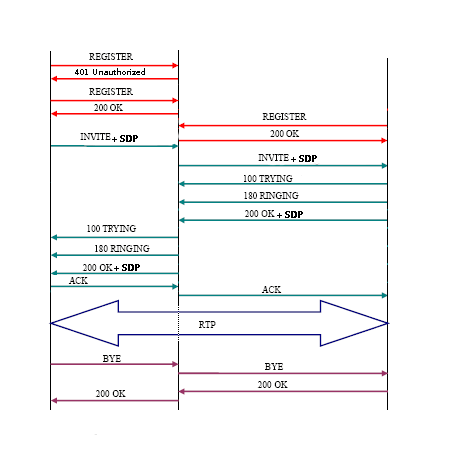
\includegraphics[width=15cm, keepaspectratio]{img/resultados/Secuencia_Paquetes.png}
  \caption{Secuencia del intercambio de paquetes}
  \label{fig:Secuencia_Paquetes_intro}
\end{figure}

\section{Estructura de la memoria}
\label{sec:estructura}
Esta sección describe la estructura organizativa de la memoria, proporcionando una visión 
general de cada uno de los capítulos principales que componen este trabajo de fin de grado. 
La estructura está diseñada para desarrollar gradualmente el tema, desde la introducción y 
los fundamentos teóricos hasta la implementación práctica y la evaluación de los resultados.

\begin{itemize}
  \item \textbf{Capítulo 1: Introducción} - Se presenta una introducción general del proyecto, estableciendo el contexto y 
  la motivación del estudio.
  
  \item \textbf{Capítulo~\ref{chap:objetivos}: Objetivos} - Detalla los objetivos generales y específicos que guían el desarrollo del proyecto.
  
  \item \textbf{Capítulo~\ref{chap:estado}: Estado del Arte} - Se comentan todas las tecnologías, herramientas y accesorios necesarios
 para el desarrollo y funcionamiento de este proyecto.
  
  \item \textbf{Capítulo~\ref{chap:diseno}: Diseño e implementación} - Describe los métodos utilizados para desarrollar el sistema de comunicación, 
  incluyendo el diseño, las herramientas y tecnologías empleadas.
  
  \item \textbf{Capítulo~\ref{chap:resultados}: Resultados} - Presenta los resultados obtenidos a través de la implementación del sistema.
  
  \item \textbf{Capítulo~\ref{chap:conclusiones}: Conclusiones} - Ofrece un desarrollo de las conclusiones extraídas y 
  las recomendaciones para investigaciones futuras.
\end{itemize}

Cada capítulo está diseñado para construir sobre la información presentada en los anteriores, asegurando un 
flujo lógico y coherente a lo largo de la memoria.




%%%%%%%%%%%%%%%%%%%%%%%%%%%%%%%%%%%%%%%%%%%%%%%%%%%%%%%%%%%%%%%%%%%%%%%%%%%%%%%%
%%%%%%%%%%%%%%%%%%%%%%%%%%%%%%%%%%%%%%%%%%%%%%%%%%%%%%%%%%%%%%%%%%%%%%%%%%%%%%%%
% OBJETIVOS %
%%%%%%%%%%%%%%%%%%%%%%%%%%%%%%%%%%%%%%%%%%%%%%%%%%%%%%%%%%%%%%%%%%%%%%%%%%%%%%%%

\cleardoublepage % empezamos en página impar
\chapter{Objetivos} % título del capítulo (se muestra)
\label{chap:objetivos} % identificador del capítulo (no se muestra, es para poder referenciarlo)

\section{Objetivo general} % título de sección (se muestra)
\label{sec:objetivo-general} % identificador de sección (no se muestra, es para poder referenciarla)

El objetivo principal es construir una representación visual y funcional de los flujos de señalización y 
datos utilizando la biblioteca de JavaScript Three.js, junto con tecnologías de VR para facilitar la interacción con la simulación. 
Se busca demostrar cómo se inicia, se mantiene y se termina una sesión de comunicación, siguiendo los estándares del protocolo SIP, 
y cómo los paquetes RTP son utilizados para el intercambio efectivo de datos multimedia.


\section{Objetivos específicos}
\label{sec:objetivos-especificos}
Para cumplir con el objetivo general de desarrollar una representación visual y funcional de los flujos de señalización 
y datos en un entorno de realidad virtual, se establecen los siguientes objetivos específicos:

\begin{enumerate}
\item Diseñar e implementar un modelo virtual en 3D que simule el entorno de una red de comunicaciones, empleando la biblioteca Three.js.
\item Integrar tecnologías de realidad virtual para facilitar una experiencia inmersiva y 
la interacción del usuario con el modelo de simulación.
\item Desarrollar una interfaz de usuario que permita la visualización y manipulación de los procesos de 
señalización y transmisión de datos, acorde con el protocolo SIP.
\item Implementar la lógica para simular el flujo de mensajes SIP, incluyendo el registro de usuarios, la iniciación y 
recepción de llamadas.
\item Simular la transmisión de datos multimedia a través de paquetes RTP, mostrando la secuencia de envío y recepción en tiempo real.
\item Crear un sistema de retroalimentación visual que indique el estado de las comunicaciones, incluyendo errores y mensajes de confirmación.
\end{enumerate}


%%%%%%%%%%%%%%%%%%%%%%%%%%%%%%%%%%%%%%%%%%%%%%%%%%%%%%%%%%%%%%%%%%%%%%%%%%%%%%%%
%%%%%%%%%%%%%%%%%%%%%%%%%%%%%%%%%%%%%%%%%%%%%%%%%%%%%%%%%%%%%%%%%%%%%%%%%%%%%%%%
% ESTADO DEL ARTE %
%%%%%%%%%%%%%%%%%%%%%%%%%%%%%%%%%%%%%%%%%%%%%%%%%%%%%%%%%%%%%%%%%%%%%%%%%%%%%%%%

\cleardoublepage
\chapter{Estado del arte}
\label{chap:estado}

En este capítulo se explicarán todas las tecnologías, herramientas y accesorios necesarios para el desarrollo, lo cual es crucial para 
comprender los fundamentos que hacen posible nuestros marcos de desarrollo. Todo esto se debe a avances significativos en tecnologías como WebVR. 
Hasta hace poco, las experiencias de VR en la web eran limitadas debido a las restricciones de ancho de banda para la transmisión de datos. 
Sin embargo, esta situación ha cambiado drásticamente. Proyectos como Google Stadia o Steam VR ejemplifican cómo la ejecución de experiencias de VR 
desde servidores remotos ha transformado la forma en que interactuamos con la realidad virtual en la web.

\bigskip

WebVR está compuesta por librerías de JavaScript que garantizan la compatibilidad con los navegadores. Además, cada navegador puede implementar 
modificaciones para adaptarse a sus particularidades.

\bigskip

Una de las fortalezas de WebVR es su naturaleza de código abierto, lo que hace que su desarrollo sea accesible para todos.

\bigskip

Además, WebVR realiza un seguimiento del rendimiento, ya que la realidad virtual puede causar malestar si la tasa de fotogramas es baja. En dispositivos 
móviles, la frecuencia de actualización es de 60Hz y 60fps, mientras que en computadoras es de 90Hz.

\bigskip

En términos de accesibilidad, WebVR se destaca, ya que no se requieren habilidades técnicas avanzadas para su uso. Con solo tener un ordenador, 
un navegador compatible y hardware de soporte (como gafas VR), puedes disfrutar de una experiencia de VR con solo un clic.

\bigskip

En cuanto a la compatibilidad, WebVR es compatible con todos los navegadores modernos (Chrome, Firefox, Safari, Edge), y también con la realidad 
aumentada y mixta.

\bigskip

Finalmente, WebVR se integra con la nube, lo que es una ventaja cada vez más demandada en la actualidad.


\section{Lenguajes de marcado y programación} 
\label{sec:lenguajes}

\begin{itemize}
  \item \textbf{HTML:} Lenguaje estándar para crear páginas web, define la estructura y el contenido utilizando etiquetas
  \footnote{\url{https://developer.mozilla.org/es/docs/Web/HTML}}.
    \begin{itemize}
        \item Funcionalidades clave:
        \begin{itemize}
            \item Definición de la estructura de una página web mediante elementos como encabezados, párrafos, listas, etc.
            \item Incorporación de contenido multimedia, como imágenes, videos y audio.
            \item Creación de formularios interactivos para la recopilación de datos.
        \end{itemize}
    \end{itemize}
  
  \item \textbf{JavaScript:} Lenguaje de programación utilizado en desarrollo web para agregar interactividad y dinamismo a las páginas
  \footnote{\url{https://developer.mozilla.org/en-US/docs/Web/JavaScript}}.
    \begin{itemize}
        \item Funcionalidades clave:
        \begin{itemize}
            \item Manipulación y modificación del contenido HTML y CSS en tiempo real.
            \item Gestión de eventos del navegador, como clics de ratón, pulsaciones de teclas y desplazamientos.
            \item Comunicación asincrónica con el servidor mediante peticiones AJAX.
        \end{itemize}
    \end{itemize}
  
  \item \textbf{TeX:} Sistema de composición tipográfica utilizado principalmente para la creación de documentos científicos y técnicos de calidad
  \footnote{\url{https://www.latex-project.org/}}.
    \begin{itemize}
        \item Funcionalidades clave:
        \begin{itemize}
            \item Tipografía de alta calidad para la composición de documentos científicos, libros y artículos académicos.
            \item Soporte avanzado para escritura matemática y fórmulas complejas.
            \item Personalización detallada de la apariencia del documento mediante la definición de estilos y formatos.
        \end{itemize}
    \end{itemize}
\end{itemize}

\begin{figure}
  \centering
  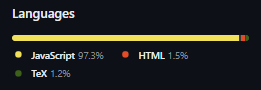
\includegraphics[width=6cm, keepaspectratio]{img/lenguajes.png}
  \caption{Porcentaje de lenguajes usados.}
  \label{fig:lenguajes}
\end{figure}


\section{Importaciones de bibliotecas JavaScript} 
\label{sec:importaciones}

En esta sección, se detallan las bibliotecas JavaScript utilizadas en el proyecto para facilitar la creación y renderización de gráficos en 3D, 
así como la integración de funcionalidades de realidad virtual (VR) y realidad extendida (XR).

\begin{itemize}
  \item \textbf{THREE.js:}
    \begin{itemize}
      \item \textbf{Descripción:} THREE.js es una biblioteca de código abierto que proporciona una amplia gama de herramientas y funciones para trabajar 
      con gráficos en 3D en el navegador web. Permite la creación y manipulación de escenas 3D, modelos tridimensionales, materiales, luces y 
      cámaras~\cite{Documentacion_Three.js}.
      \item \textbf{Funcionalidades clave:}
      \begin{itemize}
        \item Renderización de gráficos 3D en tiempo real.
        \item Creación y manipulación de modelos tridimensionales.
        \item Implementación de efectos visuales y materiales realistas.
        \item Gestión de luces y sombras en la escena.
        \item Control de la cámara para la navegación en entornos 3D.
      \end{itemize}
    \end{itemize}
  
\bigskip

  \item \textbf{VRButton.js:}
    \begin{itemize}
      \item \textbf{Descripción:} VRButton.js es un módulo de THREE.js diseñado específicamente para simplificar la integración de funcionalidades de realidad 
      virtual en aplicaciones web. Proporciona una interfaz para la activación y desactivación de la visualización en VR, así como para la detección de dispositivos 
      de VR compatibles~\cite{Documentacion_VR}.
      \item \textbf{Funcionalidades clave:}
      \begin{itemize}
        \item Integración de botones para activar/desactivar la visualización en VR.
        \item Detección automática de dispositivos de VR compatibles.
        \item Facilita la creación de experiencias inmersivas en la web.
      \end{itemize}
    \end{itemize}
  
  \item \textbf{XRControllerModelFactory.js:}
    \begin{itemize}
      \item \textbf{Descripción:} XRControllerModelFactory.js es otro módulo de THREE.js que ofrece una fábrica para la creación de modelos de controladores de 
      realidad extendida (XR). Estos modelos son representaciones visuales de los controladores utilizados por los usuarios dentro del entorno virtual y pueden 
      personalizarse según las necesidades del proyecto~\cite{Documentacion_WebXR}.
      \item \textbf{Funcionalidades clave:}
      \begin{itemize}
        \item Creación de modelos de controladores XR para representar dispositivos de VR/AR.
        \item Personalización de la apariencia y comportamiento de los modelos de controladores.
        \item Integración fluida con aplicaciones de XR.
      \end{itemize}
    \end{itemize}
  
  \item \textbf{Stats.js:}
    \begin{itemize}
      \item \textbf{Descripción:} Stats.js es un módulo de THREE.js que proporciona una herramienta para monitorear el rendimiento de aplicaciones web 3D en tiempo real. 
      Permite realizar un seguimiento de métricas importantes, como los cuadros por segundo (FPS), el uso de memoria y el tiempo de procesamiento de cuadros~\cite{Statsjs}.
      \item \textbf{Funcionalidades clave:}
      \begin{itemize}
        \item Monitoreo del rendimiento en tiempo real de aplicaciones web 3D.
        \item Visualización de métricas como FPS y uso de memoria.
        \item Ayuda en la identificación y solución de cuellos de botella de rendimiento.
      \end{itemize}
    \end{itemize}
  
  \item \textbf{OrbitControls.js:}
    \begin{itemize}
      \item \textbf{Descripción:} OrbitControls.js es un módulo de THREE.js que proporciona controles de órbita para permitir al usuario manipular la cámara 
      en una escena 3D de manera interactiva. Permite rotar, acercar y alejar la vista de la escena, lo que mejora la experiencia de navegación~\cite{Documentacion_Controls}.
      \item \textbf{Funcionalidades clave:}
      \begin{itemize}
        \item Control de la cámara para la navegación interactiva en entornos 3D.
        \item Rotación, acercamiento y alejamiento suaves de la cámara.
        \item Personalización de la sensibilidad y restricciones de los controles.
      \end{itemize}
    \end{itemize}
\end{itemize}


\section{Herramientas de desarrollo} 
\label{sec:herramientas}

\begin{itemize}
  \item \textbf{FireFox:} Navegador web de código abierto conocido por su enfoque en la privacidad y la personalización. Destaca por su capacidad 
  para bloquear rastreadores de anuncios y proteger la privacidad del usuario. Además, ofrece una amplia gama de complementos y extensiones que permiten 
  personalizar la experiencia de navegación según las preferencias del usuario~\cite{Firefox}.
  
  \item \textbf{VisualStudioCode:} Editor de código fuente de Microsoft altamente personalizable y de código abierto, conocido por su rendimiento y amplia gama 
  de extensiones. Es ampliamente utilizado por desarrolladores de software debido a su interfaz intuitiva, funcionalidades avanzadas de edición de código y soporte 
  para una variedad de lenguajes de programación y tecnologías~\cite{Vscode}.
  
  \item \textbf{GitHub:} Plataforma de desarrollo colaborativo de software basada en la nube, que permite a los desarrolladores alojar, revisar, colaborar y desplegar 
  proyectos de software, incluidas aplicaciones web, de manera eficiente y transparente. Es ampliamente utilizado en la comunidad de desarrollo de software para gestionar 
  versiones de código, coordinar el trabajo en equipo y facilitar la contribución de la comunidad al código abierto~\cite{Github}.
  
  \item \textbf{Oculus Quest 2:} Gafas de realidad virtual autónomas producidas por Oculus (una subsidiaria de Facebook), conocidas por su alta calidad y facilidad de uso. 
  Estas gafas fueron proporcionadas por la universidad para el desarrollo del proyecto. Ofrecen una experiencia inmersiva de realidad virtual sin necesidad de estar 
  conectadas a un PC o consola, lo que las hace ideales para el desarrollo y la experiencia de usuario en entornos de realidad virtual~\cite{Oculus}.
  
  \item \textbf{Web XR API Emulator:} Herramienta de desarrollo que permite probar y depurar experiencias de realidad virtual y aumentada basadas en WebXR directamente 
  en el navegador web. Facilita a los desarrolladores la creación y prueba de contenido de realidad virtual y aumentada sin necesidad de hardware especializado, lo que 
  agiliza el proceso de desarrollo y depuración de aplicaciones basadas en WebXR~\cite{Webxrapiemulator}.
  
\end{itemize}


\section{Protocolos visualizados} 
\label{sec:protocolos}

\section{Herramientas de desarrollo} 
\label{sec:herramientas}

En esta sección, se detallan los protocolos utilizados en el desarrollo del proyecto, los cuales son esenciales para la comunicación en tiempo real y 
la transmisión de datos multimedia.

\begin{itemize}
  \item \textbf{SIP (Session Initiation Protocol):}
    \begin{itemize}
      \item \textbf{Descripción:} SIP es un protocolo de señalización utilizado para iniciar, mantener y finalizar sesiones de comunicación en tiempo real, 
      como llamadas de voz y video. Es un protocolo de capa de aplicación que puede gestionar la creación, modificación y finalización de sesiones 
      con uno o más participantes~\cite{Documentacion_SIP}.
      \item \textbf{Funcionalidades clave:}
      \begin{itemize}
        \item Establecimiento y finalización de llamadas de voz y video.
        \item Modificación de sesiones en tiempo real añadiendo o eliminando participantes.
        \item Interoperabilidad con otros protocolos de comunicación.
        \item Soporte para autenticación y cifrado de comunicaciones.
      \end{itemize}
    \end{itemize}
  
  \item \textbf{RTP (Real-time Transport Protocol):}
    \begin{itemize}
      \item \textbf{Descripción:} RTP es un protocolo de red diseñado para la entrega de datos en tiempo real, como audio y video, a través de redes IP. 
      Es ampliamente utilizado en aplicaciones que requieren transmisión continua de datos multimedia~\cite{Documentacion_RTP}.
      \item \textbf{Funcionalidades clave:}
      \begin{itemize}
        \item Transmisión de datos en tiempo real (audio y video).
        \item Sincronización de flujos multimedia.
        \item Detección y corrección de pérdidas de paquetes.
        \item Extensibilidad para soportar nuevos códecs y funcionalidades.
      \end{itemize}
    \end{itemize}
  
  \item \textbf{SDP (Session Description Protocol):}
    \begin{itemize}
      \item \textbf{Descripción:} SDP es un formato estándar para describir los detalles de las sesiones multimedia con el objetivo de iniciar y gestionar comunicaciones. 
      Este protocolo es utilizado comúnmente junto con SIP para negociar los parámetros de la sesión, como los códecs a utilizar, 
      las direcciones IP y los puertos~\cite{Documentacion_SDP}.
      \item \textbf{Funcionalidades clave:}
      \begin{itemize}
        \item Descripción de los parámetros de la sesión multimedia.
        \item Negociación de capacidades de comunicación entre los participantes.
        \item Integración con protocolos de señalización como SIP.
        \item Formato flexible para adaptarse a diferentes configuraciones de red.
      \end{itemize}
    \end{itemize}
  
\end{itemize}



%%%%%%%%%%%%%%%%%%%%%%%%%%%%%%%%%%%%%%%%%%%%%%%%%%%%%%%%%%%%%%%%%%%%%%%%%%%%%%%%
%%%%%%%%%%%%%%%%%%%%%%%%%%%%%%%%%%%%%%%%%%%%%%%%%%%%%%%%%%%%%%%%%%%%%%%%%%%%%%%%
% DISEÑO E IMPLEMENTACIÓN %
%%%%%%%%%%%%%%%%%%%%%%%%%%%%%%%%%%%%%%%%%%%%%%%%%%%%%%%%%%%%%%%%%%%%%%%%%%%%%%%%

\cleardoublepage
\chapter{Diseño e implementación}
\label{chap:diseno}

En este capítulo se detalla el desarrollo del proyecto, incluyendo su estructura, los componentes en el entorno 
inmersivo, su funcionamiento, y las interacciones implementadas.


\section{Arquitectura general} 
\label{sec:arquitectura}

El proyecto se estructura en cinco componentes enlazados entre si, representados en la figura~\ref{fig:arquitectura}. Estos componentes serán explicados a continuación:

\begin{itemize}
  \item \textbf{index.html:} Representamos la estructura básica de una página web para una experiencia de realidad virtual (VR). 
  Se define un documento HTML con metadatos y referencias a archivos externos, incluyendo la biblioteca Three.js para gráficos 3D. 
  
  Además, se importa un módulo de JavaScript que inicializa la aplicación VR, creando una instancia de la clase App y asignándola a la ventana del navegador. 
  
  Este archivo proporciona una base para el desarrollo de aplicaciones de realidad virtual en la web.
  
  \item \textbf{app.js:} Este script es una aplicación que utiliza la biblioteca Three.js para crear una escena 3D interactiva. Que realiza:
    
    \begin{enumerate}
      \item Importa las bibliotecas necesarias de Three.js para crear la escena.
      \item Carga varias texturas de imágenes para aplicarlas a los materiales de los objetos en la escena.
      \item Define algunas variables y objetos necesarios para el funcionamiento de la aplicación.
      \item Crea una clase App que inicializa la escena, la cámara, la iluminación y los controles.
      \item Dentro de la clase App, hay métodos para manejar el control de los dispositivos de entrada de VR, como los controladores y sus eventos.
      \item Contiene un método para construir los modelos de los controladores de VR.
      \item Otro método se encarga de manejar la lógica de la animación y la interacción del usuario con la escena.
      \item Y finalmente, tenemos un método de renderizado que se ejecuta en bucle y actualiza la escena en cada fotograma.
    \end{enumerate}

  \item \textbf{imágenes:} En la arquitectura del proyecto, tenemos una carpeta llamada imagenes que contiene todas las imágenes utilizadas en la aplicación. 
  Dentro de esta carpeta, tenemos subcarpetas para organizar las imágenes de acuerdo con su propósito.

  Cada imagen se carga en la aplicación utilizando el constructor THREE.TextureLoader().load(), 
  proporcionando la ruta relativa desde el punto donde se está ejecutando el código hacia la ubicación de la imagen en la estructura de carpetas.

  \item \textbf{sceneObjets:} Este archivo es un módulo de funciones que proporciona diferentes objetos tridimensionales (3D) utilizando la biblioteca Three.js. 
  Cada función devuelve un objeto con geometría y material específicos.

  \begin{enumerate}
    \item \textbf{Sphere:} Devuelve una esfera roja con una geometría esférica y un material básico.
    \item \textbf{Side:} Devuelve un objeto rectangular con una textura proporcionada, usado como pared en la escena.
    \item \textbf{Box:} Devuelve una caja con una textura proporcionada, usado como UA y Proxy en la escena.
    \item \textbf{Wall:} Devuelve un plano grande con una textura proporcionada, usado como pantalla en la escena.
    \item \textbf{Logo:} Devuelve un plano con una textura proporcionada, representando logotipo.
    \item \textbf{Floor:} Devuelve un plano grande con una textura proporcionada, usado para el suelo de la escena.
  \end{enumerate}

  Cada función utiliza diferentes geometrías y materiales para crear los objetos 3D. 
  También configura propiedades específicas de los materiales, como envoltura de textura y repetición.
  
  \item \textbf{jsm:} Esta carpeta contiene módulos JavaScript utilizados en el proyecto. Estos módulos son archivos independientes que proporcionan funcionalidades específicas para la aplicación. 
  Aquí está la estructura de la carpeta:

  \begin{enumerate}
    \item \textbf{build:} En esta subcarpeta se encuentran los archivos de construcción de la biblioteca Three.js, 
    que proporcionan la funcionalidad principal de renderización en 3D. El archivo principal utilizado es three.module.js, 
    que importa todas las funcionalidades esenciales de Three.js.
    \item \textbf{webxr:} Aquí están los módulos relacionados con WebXR, una API que permite crear experiencias de realidad virtual (VR) y realidad aumentada (AR) en el navegador. 
    Por ejemplo, VRButton.js proporciona un botón para activar la experiencia de realidad virtual, mientras que XRControllerModelFactory.js 
    permite crear modelos visuales para los controladores de VR.
    \item \textbf{libs:} Esta subcarpeta contiene bibliotecas adicionales utilizadas en el proyecto. 
    En particular, stats.module.js proporciona una herramienta para medir el rendimiento de la aplicación 
    mediante la visualización de estadísticas, como el número de fotogramas por segundo.
    \item \textbf{controls:} Aquí están los módulos relacionados con el control de la cámara y la escena en la aplicación. 
    Por ejemplo, OrbitControls.js proporciona controles para permitir al usuario mover y rotar la cámara 
    alrededor de la escena, lo que facilita la navegación en entornos 3D.
  \end{enumerate}

  Por lo tanto, la carpeta jsm organiza los módulos JavaScript utilizados en el proyecto, 
  proporcionando funcionalidades esenciales, soporte para WebXR, herramientas de medición de rendimiento y controles de cámara. 
  Estos módulos se importan en la aplicación según sea necesario para agregar las características deseadas.

\end{itemize}

\begin{figure}
  \centering
  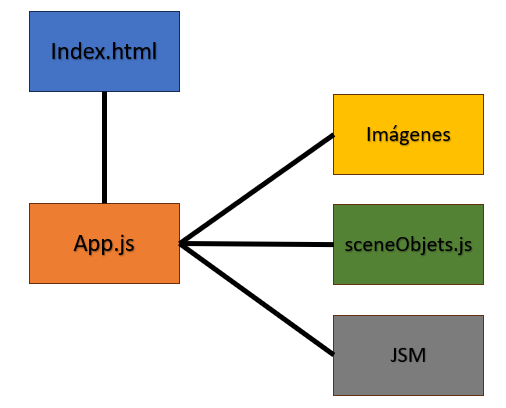
\includegraphics[width=12cm, keepaspectratio]{img/estructura.png}
  \caption{Estructura del proyecto}
  \label{fig:arquitectura}
\end{figure}


\section{Escena} 
\label{sec:escena}

La escena virtual implementada se desarrolla utilizando la biblioteca Three.js, 
que permite la creación de gráficos 3D en un entorno web. Este proyecto configura un entorno interactivo 
que simula un sistema de comunicación, donde se pueden visualizar los intercambios de mensajes entre diferentes usuarios y un proxy.
Esta escena es representada en la figura~\ref{fig:escena}.

\bigskip

\textbf{Estructura básica}

\begin{itemize}
  \item \textbf{Cámara y Controles:} La cámara se configura con una perspectiva que permite al usuario tener una vista adecuada del entorno virtual. 
  Se utiliza OrbitControls para permitir al usuario interactuar con la vista, rotando y acercando/alejando la escena.
  
  \item \textbf{Iluminación:} Se añade iluminación hemisférica para simular una luz suave y direccional 
  para destacar objetos específicos dentro de la escena.

  \item \textbf{Renderizado:} Se establece un renderizado con antialiasing para mejorar la calidad visual de los bordes de los objetos en la escena.
  
\end{itemize}

\textbf{Objetos en la escena}

\begin{itemize}
  \item \textbf{Suelo y paredes:} Se utilizan texturas cargadas para crear un suelo y paredes que encierran la escena, proporcionando un fondo estático.
  
  \item \textbf{Objetos interactivos:} Se crean varias cajas y esferas que representan a diferentes usuarios (UA1, UA2) y un proxy. 
  Estos objetos se pueden interactuar mediante eventos controlados por los controladores de realidad virtual.

  \item \textbf{Indicadores visuales:} Se utilizan logos y texturas para indicar estados como start y stop, mostrando visualmente el flujo de la simulación.
  
\end{itemize}

\textbf{Interacción y dinámica}

\begin{itemize}
  \item \textbf{Inicio de eventos:} La interacción comienza cuando el usuario activa controles específicos en los controladores de realidad virtual. 
  Esto puede alterar el estado de los objetos (por ejemplo, cambiar el color para indicar actividad) y cambiar texturas que 
  representan diferentes mensajes enviados y recibidos en la comunicación.
  
  \item \textbf{Simulación de mensajes:} Los objetos esféricos se mueven entre las cajas para simular el envío de mensajes. 
  La ruta y la dirección de estos objetos dependen de las interacciones del usuario y el flujo del protocolo simulado.

  \item \textbf{Animación de paquetes RTP:} En ciertos puntos, esferas adicionales se mueven para simular la transmisión de paquetes RTP, 
  indicando el intercambio de media en una llamada establecida.
  
\end{itemize}


\textbf{Implementación}

\begin{itemize}
  \item \textbf{Controladores XR:} Se configuran controladores para manejar la interacción en un entorno de realidad extendida (XR). 
  Esto incluye la gestión de eventos de selección y conexión de dispositivos.
  
  \item \textbf{Animación y actualización de la escena:} La animación de la escena se inicia con los controladores, simulando el intercambio de 
  paquetes mediante objetos esféricos. Estos objetos siguen una ruta y dirección determinadas por el estado actual del sistema, representando de 
  manera visual el flujo del protocolo de comunicación.

  \item \textbf{Animación de paquetes RTP:} La lógica para mover objetos y actualizar estados se ejecuta dentro de un bucle 
  de animación que recalcula posiciones y estados basados en la interacción del usuario.
  
\end{itemize}

\begin{figure}
  \centering
  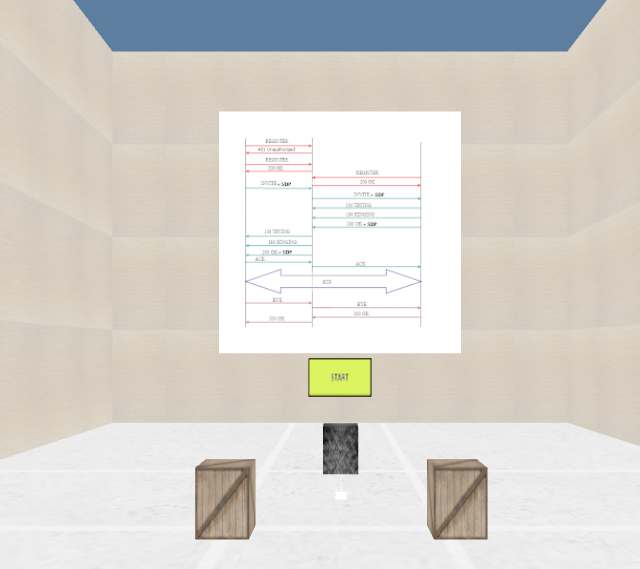
\includegraphics[width=9cm, keepaspectratio]{img/escena.png}
  \caption{Escena del proyecto}
  \label{fig:escena}
\end{figure}


\section{Controles de realidad virtual}
\label{sec:controles_vr}

La implementación de controles de realidad virtual en la aplicación proporciona una interfaz interactiva que mejora significativamente la experiencia del usuario, 
permitiendo una manipulación intuitiva y directa de la escena virtual.

\subsection{Configuración de los controladores VR}
\label{subsec:configuracion_controladores_vr}

Los controladores VR son dispositivos físicos que los usuarios sostienen en sus manos y que detectan sus movimientos y gestos en el espacio tridimensional. 
Estos están equipados con una variedad de sensores y botones que permiten una gama amplia de interacciones:

\begin{itemize}
  \item \textbf{Botones y Gatillos}: Utilizados para realizar selecciones y activar eventos dentro de la aplicación. 
  Por ejemplo, un usuario puede iniciar la transmisión de mensajes al presionar el botón Start.
  \item \textbf{Sensores de Movimiento}: Capturan el posicionamiento y la orientación de las manos del usuario, 
  permitiendo manipular objetos o navegar por la escena con movimientos naturales.
\end{itemize}

\begin{figure}
  \centering
  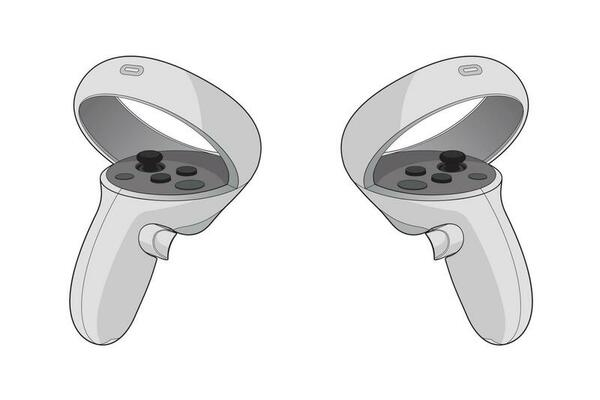
\includegraphics[width=6cm, keepaspectratio]{img/controlador.png}
  \caption{Controlador VR}
  \label{fig:controlador}
\end{figure}


\subsection{Interacción mediante controladores VR}
\label{subsec:interaccion_controladores_vr}

La interacción con la escena se realiza a través de los controladores VR de la siguiente manera:

\begin{itemize}
  \item \textbf{Selección y Manipulación}: Los usuarios apuntan a objetos virtuales con los controladores y utilizan 
  botones para seleccionarlos. Esto puede incluir activar elementos dentro de la escena.
  \item \textbf{Navegación}: Mediante el uso del gatillo en los controladores, 
  los usuarios pueden desplazarse por la escena virtual, acercándose o alejándose de los objetos o desplazándose lateralmente.
  \item \textbf{Interacción Contextual}: La aplicación cambia la funcionalidad de la escena 
  basándose en el estado del objeto con el que el usuario está interactuando, 
  cambiando modos de visualización o ajustando parámetros específicos de los objetos.
\end{itemize}

\subsection{Implementación técnica}
\label{subsec:implementacion_tecnica_vr}

La implementación técnica de los controladores VR en la aplicación utiliza la API de WebXR, integrada con Three.js, para gestionar la entrada 
de los dispositivos de realidad virtual. El código configura cada controlador para responder a eventos como `selectstart` y `selectend`, 
lo que permite detectar interacciones como pulsaciones de botones y liberaciones. Adicionalmente, se emplean rayos virtuales `raycasting` 
para determinar qué objetos están siendo apuntados por los controladores, facilitando así una interacción precisa~\cite{Using_a_WebXR_controller_using_Three.JS}.


En la implementación de la aplicación, hacemos un uso específico de los botones trigger de los controladores VR para facilitar una interacción 
intuitiva y efectiva dentro del entorno virtual. Cada trigger tiene un propósito bien definido que mejora la experiencia del 
usuario y la funcionalidad de la aplicación:

\begin{itemize}
  \item \textbf{Trigger del controlador izquierdo}: Este botón se utiliza para la navegación dentro de la escena. Al presionar el trigger del controlador izquierdo, 
  el usuario puede desplazarse hacia donde esté mirando con las gafas de realidad virtual, lo que permite una navegación intuitiva y natural. 
  Esta funcionalidad es fundamental para explorar diferentes áreas de la escena de manera fluida.
  
  \item \textbf{Trigger del controlador derecho}: El trigger del controlador derecho está configurado para interactuar con objetos 
  específicos de la escena. Cuando se presiona este botón, se puede seleccionar o activar elementos dentro de la escena, 
  como iniciar una simulación, modificar parámetros de un objeto, o ejecutar acciones específicas relacionadas con los objetos con los que se interactúa. 
  Esta interacción es esencial para manipular elementos de la aplicación y para participar activamente en las simulaciones y demostraciones que se presentan en el entorno virtual.
\end{itemize}

La programación de estos triggers se realiza a través del manejo de eventos en JavaScript, utilizando la API de WebXR para detectar y responder 
a las acciones del usuario. Este diseño permite un control preciso sobre la aplicación, ofreciendo a los usuarios una manera clara y directa 
de interactuar con la interfaz y con los elementos virtuales de la escena.

\begin{figure}
  \centering
  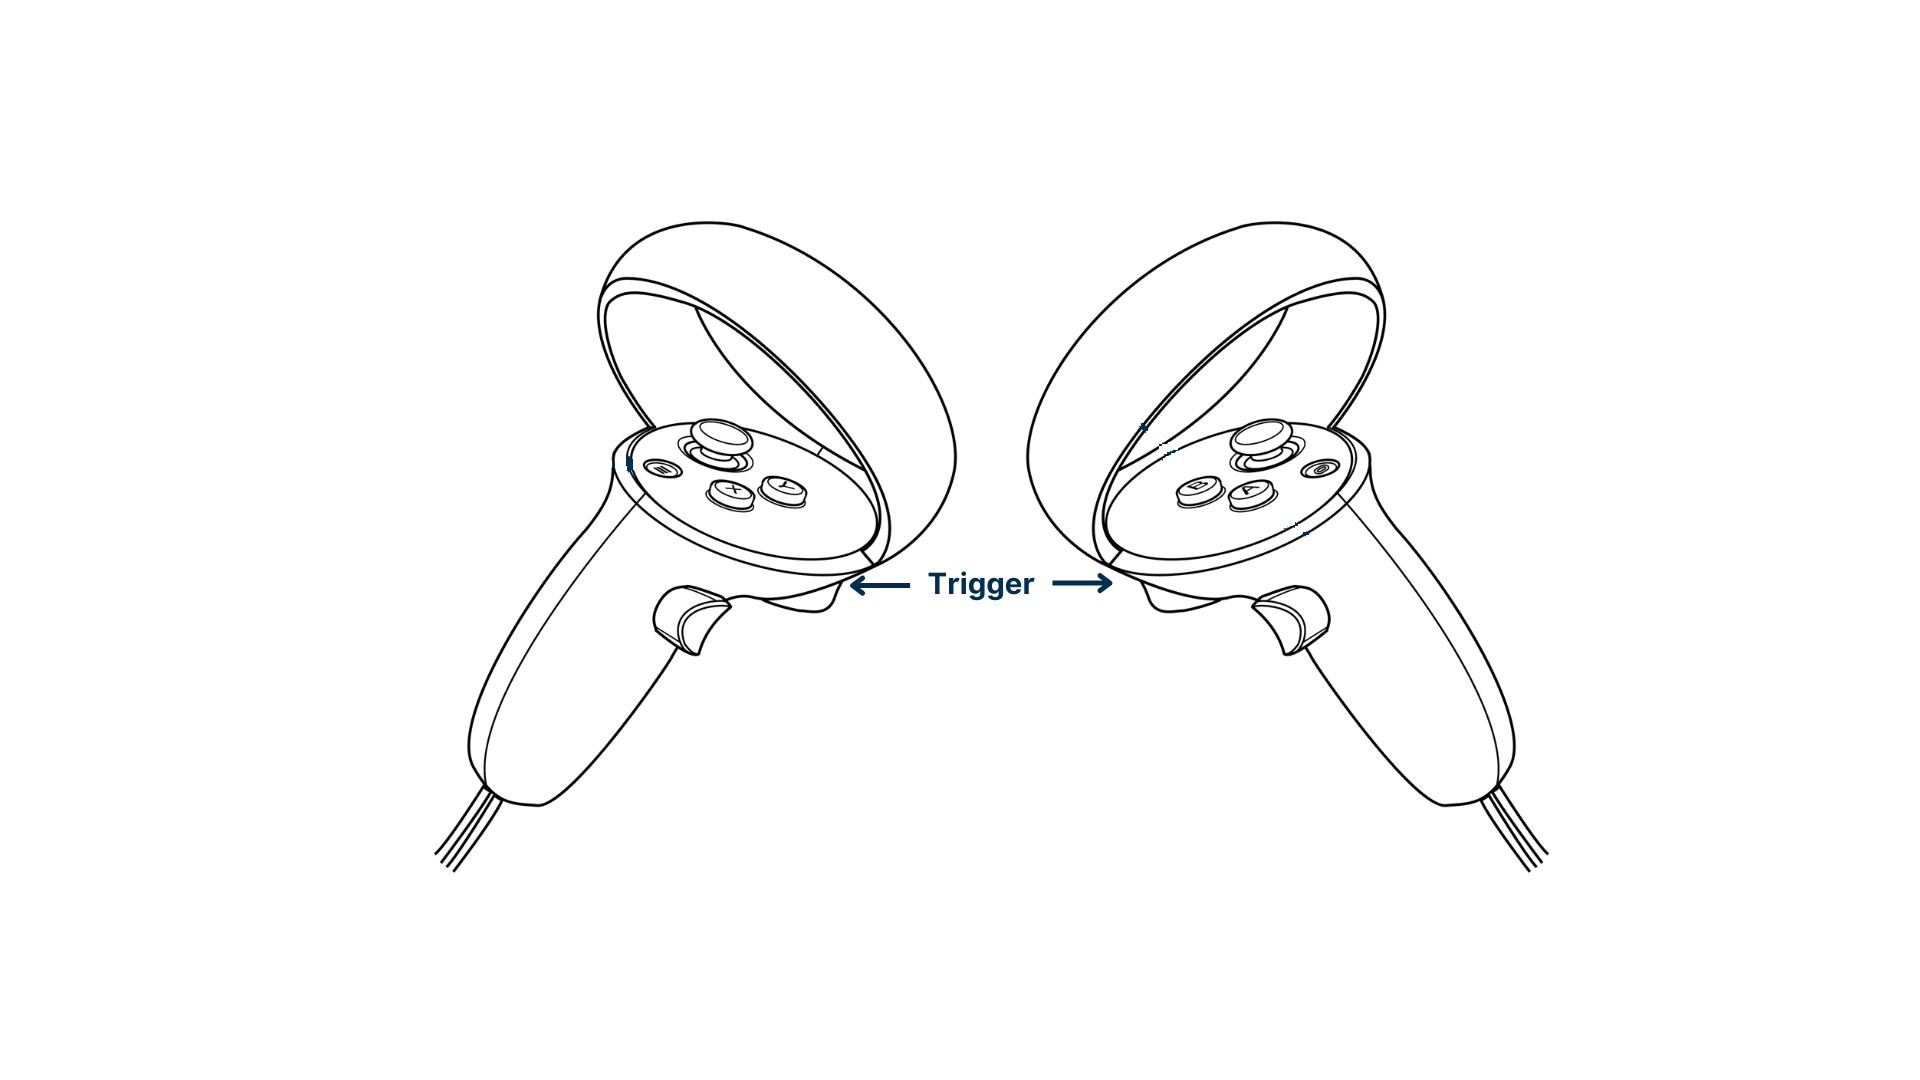
\includegraphics[width=6cm, keepaspectratio]{img/BotonesControlador.png}
  \caption{Botones controlador VR}
  \label{fig:controladorBotones}
\end{figure}


%%%%%%%%%%%%%%%%%%%%%%%%%%%%%%%%%%%%%%%%%%%%%%%%%%%%%%%%%%%%%%%%%%%%%%%%%%%%%%%%
%%%%%%%%%%%%%%%%%%%%%%%%%%%%%%%%%%%%%%%%%%%%%%%%%%%%%%%%%%%%%%%%%%%%%%%%%%%%%%%%
% RESULTADOS %
%%%%%%%%%%%%%%%%%%%%%%%%%%%%%%%%%%%%%%%%%%%%%%%%%%%%%%%%%%%%%%%%%%%%%%%%%%%%%%%%

\cleardoublepage
\chapter{Resultados}
\label{chap:resultados}

En este capítulo se presentan los resultados derivados de las interacciones con los objetos de la escena en la aplicación 
de realidad virtual desarrollada. Se describirá cómo distintas selecciones de objetos generan resultados visuales y 
funcionales diferentes, lo que demuestra la dinámica y la reactividad de la aplicación ante las acciones del usuario.

\section{Descripción de las interacciones}
\label{sec:descripcion_interacciones}
Las interacciones en la aplicación permiten a los usuarios seleccionar objetos virtuales, 
los cuales alteran el estado de la escena y desencadenan eventos específicos. 

Como se mencionó en la Sección 4.3.3, para lograr estos resultados es necesario utilizar controladores VR. 
Estos dispositivos permiten a los usuarios moverse por la escena e interactuar con los objetos de manera intuitiva y efectiva.
La selección se realiza apuntando hacia el objeto con el controlador derecho y activando el trigger.

Cada objeto tiene asociadas consecuencias específicas que se detallan a continuación:

\subsection{Interacción con UA1}
\label{subsec:objeto_ua1}

Este objeto representa un usuario dentro del entorno virtual y está visualizado como una caja 
de madera ubicada en la parte izquierda de la escena.

Al interactuar con UA1, este cambiará de color y podrán obtener dos posibles resultados, los cuales dependen 
de si el intercambio de paquetes ha sido inicializado o no.

\subsubsection{Intercambio de paquetes no iniciado}
\label{subsubsec:Intercambio_NoIniciado}
Si el intercambio de paquetes no ha sido inicializado, en la pantalla situada en la pared central se mostrarán 
los atributos del usuario en estado vacío, indicando los valores que deberían ser completados, mostrados en la figura~\ref{fig:UA1_NoIniciado}. 
Esta visualización es esencial para comprender los requisitos iniciales de configuración del usuario en la red. Estos tributos son:

\begin{itemize}
  \item \textbf{account}: [username, passwd]
  \item \textbf{uaserver}: [ip, puerto]
  \item \textbf{rtpaudio}: [puerto]
  \item \textbf{regproxy}: [ip, puerto]
  \item \textbf{log}: [path]
  \item \textbf{audio}: [path]
\end{itemize}

\begin{figure}
  \centering
  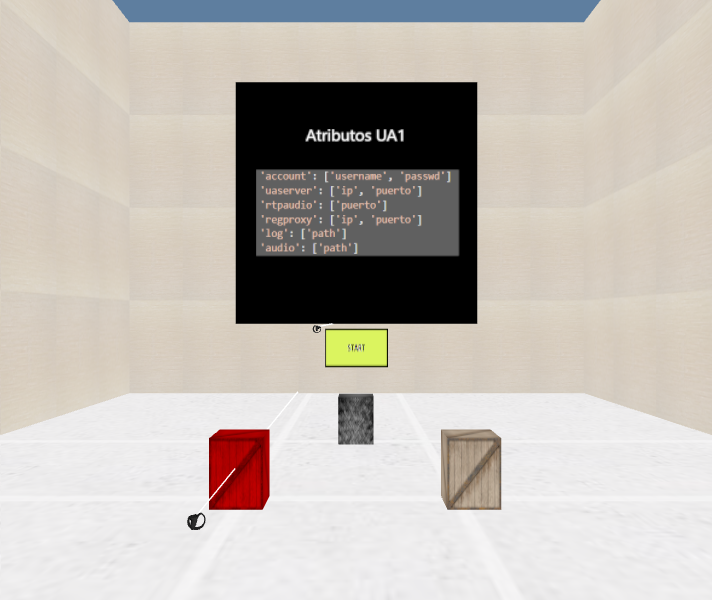
\includegraphics[width=15cm, keepaspectratio]{img/resultados/UA1_NoIniciado.png}
  \caption{Estado inicial del UA1}
  \label{fig:UA1_NoIniciado}
\end{figure}


\subsubsection{Intercambio de paquetes iniciado}
\label{subsubsec:Intercambio_Iniciado}
Una vez que el intercambio de paquetes ha sido iniciado, en la misma pantalla se 
actualizarán los atributos del usuario con valores específicos y correctos para su funcionamiento mostrados en la figura~\ref{fig:UA1_Iniciado}.  
Este cambio refleja cómo el sistema procesa y responde a las interacciones, ofreciendo un feedback visual del estado operativo del usuario.

\begin{figure}
  \centering
  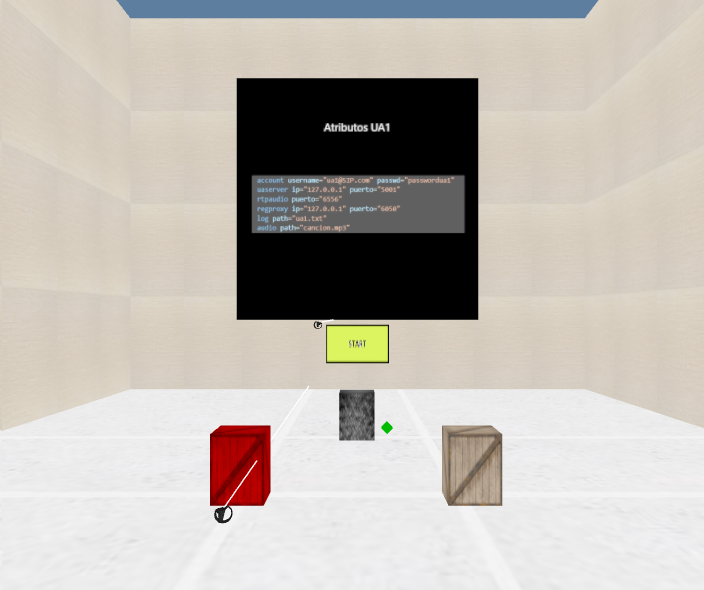
\includegraphics[width=15cm, keepaspectratio]{img/resultados/UA1_Iniciado.png}
  \caption{Atributos UA1 con valores específicos}
  \label{fig:UA1_Iniciado}
\end{figure}


\subsection{Interacción con el proxy}
\label{subsec:objeto_proxy}

Este objeto representa un servidor proxy en el entorno virtual y está visualizado como una caja con textura oscura,
ubicada en la parte central de la escena.

Al interactuar con el Proxy, este cambiará de color y dependiendo del estado de la interacción con los usuarios (UA1 y UA2), 
se pueden obtener diferentes resultados, influenciados por si el intercambio de paquetes ha sido iniciado o no.

\subsubsection{Intercambio de paquetes no iniciado}
\label{subsubsec:Proxy_Intercambio_NoIniciado}
Si el intercambio de paquetes no ha sido inicializado, la interacción con el Proxy mostrará en la pantalla sus atributos 
con la información que deben ser completados, donde no se procesan aún los paquetes, mostrados en la figura~\ref{fig:Proxy_NoIniciado}. Estos campos son:

\begin{itemize}
  \item \textbf{server}: [name, ip, puerto]
  \item \textbf{database}: [path, passwdpath]
  \item \textbf{log}: [path]
\end{itemize}

\begin{figure}
  \centering
  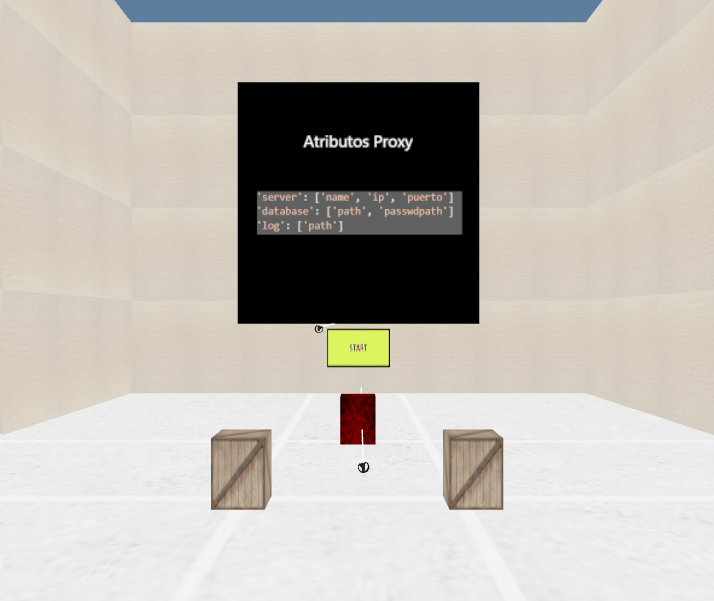
\includegraphics[width=15cm, keepaspectratio]{img/resultados/Proxy_NoIniciado.png}
  \caption{Estado inicial del Proxy}
  \label{fig:Proxy_NoIniciado}
\end{figure}

\subsubsection{Intercambio de paquetes iniciado}
\label{subsubsec:Proxy_Intercambio_Iniciado}
Una vez que el intercambio de paquetes ha sido iniciado, el Proxy procesará y dirigirá los paquetes entre los usuarios correspondientes, 
reflejando este flujo en la interfaz con actualizaciones dinámicas. Al seleccionar el Proxy se mostrarán sus atributos con valores específicos 
y correctos para su funcionamiento, mostrados en la figura~\ref{fig:Proxy_Iniciado}.

\begin{figure}
  \centering
  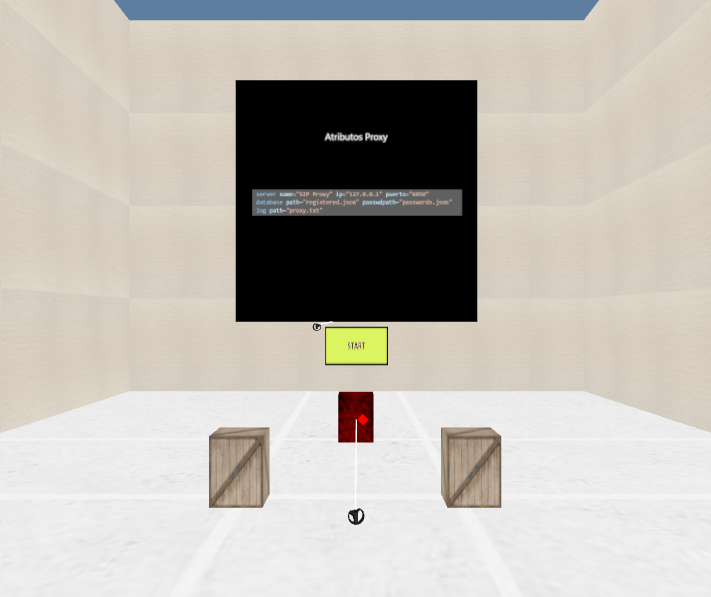
\includegraphics[width=15cm, keepaspectratio]{img/resultados/Proxy_Iniciado.png}
  \caption{Atributos Proxy con valores específicos}
  \label{fig:Proxy_Iniciado}
\end{figure}


\subsection{Interacción con UA2}
\label{subsec:objeto_ua1}

Este objeto representa un usuario dentro del entorno virtual y está visualizado como una caja 
de madera ubicada en la parte derecha de la escena.

Al interactuar con UA2, este cambiará de color y podrán obtener dos posibles resultados, los cuales dependen 
de si el intercambio de paquetes ha sido inicializado o no.

\subsubsection{Intercambio de paquetes no iniciado}
\label{subsubsec:Intercambio_NoIniciado}
Si el intercambio de paquetes no ha sido inicializado, en la pantalla situada en la pared central se mostrarán 
los atributos del usuario en estado vacío, indicando los valores que deberían ser completados, mostrados en la figura~\ref{fig:UA2_NoIniciado}. 
Esta visualización es esencial para comprender los requisitos iniciales de configuración del usuario en la red. Estos tributos son:

\begin{itemize}
  \item \textbf{account}: [username, passwd]
  \item \textbf{uaserver}: [ip, puerto]
  \item \textbf{rtpaudio}: [puerto]
  \item \textbf{regproxy}: [ip, puerto]
  \item \textbf{log}: [path]
  \item \textbf{audio}: [path]
\end{itemize}

\begin{figure}
  \centering
  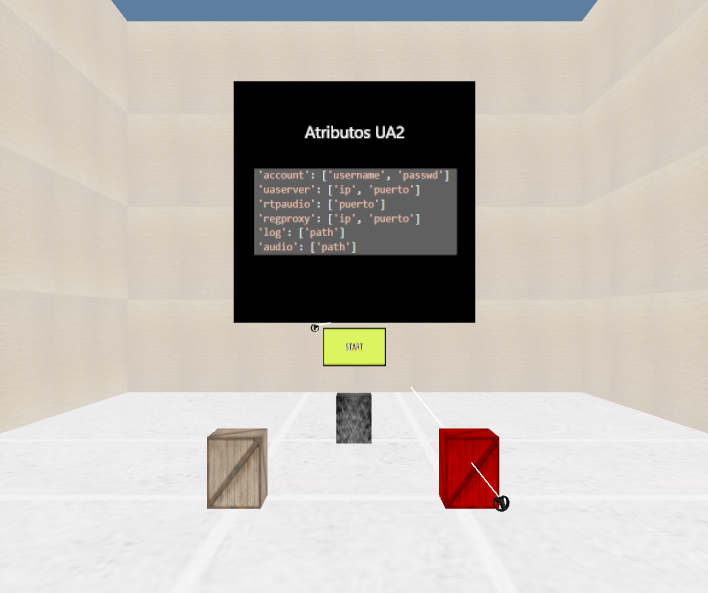
\includegraphics[width=12cm, keepaspectratio]{img/resultados/UA2_NoIniciado.png}
  \caption{Estado inicial del UA2}
  \label{fig:UA2_NoIniciado}
\end{figure}


\subsubsection{Intercambio de paquetes iniciado}
\label{subsubsec:Intercambio_Iniciado}
Una vez que el intercambio de paquetes ha sido iniciado, en la misma pantalla se 
actualizarán los atributos del usuario con valores específicos y correctos para su funcionamiento mostrados en la figura~\ref{fig:UA2_Iniciado}.  
Este cambio refleja cómo el sistema procesa y responde a las interacciones, ofreciendo un feedback visual del estado operativo del usuario.

\begin{figure}
  \centering
  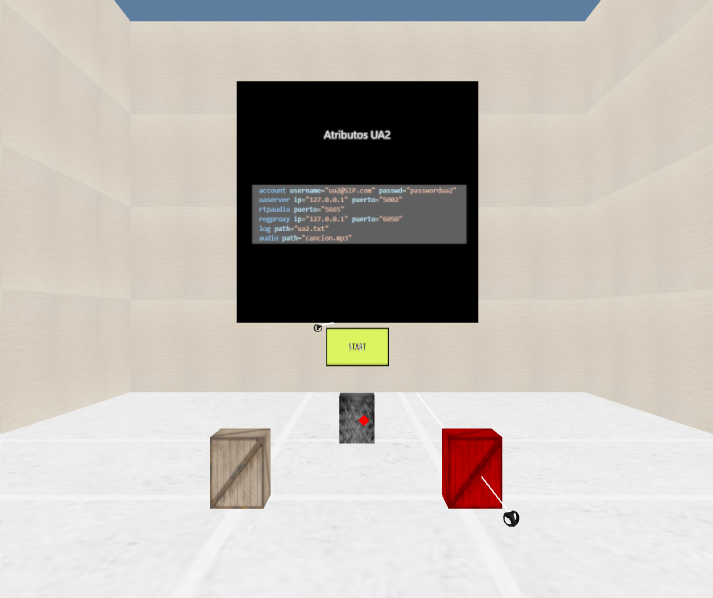
\includegraphics[width=12cm, keepaspectratio]{img/resultados/UA2_Iniciado.png}
  \caption{Atributos UA2 con valores específicos}
  \label{fig:UA2_Iniciado}
\end{figure}

\clearpage
\subsection{Interacción con paquetes}
\label{subsec:objeto_paquetes}
En el entorno de realidad virtual, los paquetes se representan en forma de esferas que simulan la transmisión de datos en una red. 
Estas esferas visualizan claramente el flujo de información, con un origen, un destino y un color claramente definidos, 
dependiendo del tipo de intercambio en el que participan.

\bigskip

Al seleccionar uno de estos paquetes, el sistema mostrará información detallada contenida en el paquete, 
incluyendo una representación visual del flujo de transmisión que indica su origen, destino y la dirección del flujo.

\bigskip

El proceso y secuencia de intercambio de paquetes en este proyecto se ilustra en la siguiente figura~\ref{fig:Secuencia_Paquetes}, donde se puede observar el orden 
específico seguido durante las simulaciones.

\bigskip

Esta figura~\ref{fig:Secuencia_Paquetes} ilustra un intercambio de mensajes de protocolo típico en una comunicación de red utilizando el Protocolo de Inicio de Sesión (SIP). 
Este diagrama de flujo representa la secuencia de mensajes entre dos usuarios que intentan establecer una comunicación, 
pasando por un proceso de registro y luego de llamada.

\begin{figure}
  \centering
  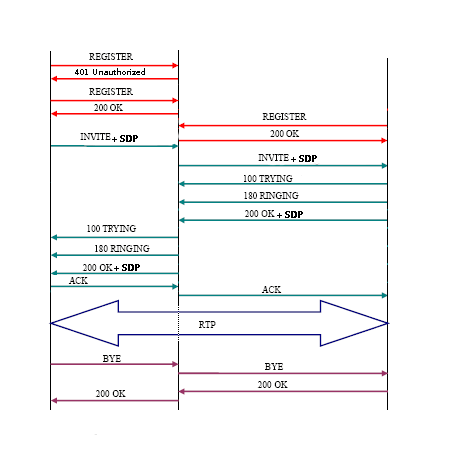
\includegraphics[width=15cm, keepaspectratio]{img/resultados/Secuencia_Paquetes.png}
  \caption{Secuencia del intercambio de paquetes}
  \label{fig:Secuencia_Paquetes}
\end{figure}



% ······································································· %
\clearpage
\subsubsection{Desglose de la secuencia de comunicación}
\label{subsubsec:secuencia_comunicacion2}

Inicialmente, el proceso comienza con un intento de registro, donde el usuario A (UA1) envía un mensaje REGISTER al servidor, 
representado en la figura~\ref{fig:01-Register_UA1}. 

Este mensaje contiene información necesaria para que el servidor registre al usuario en el sistema.
Esta información generalmente incluye el identificador del usuario, su dirección de red y otros parámetros necesarios para la autenticación y la 
configuración de la sesión.

\bigskip

\begin{figure}[H]
  \centering
  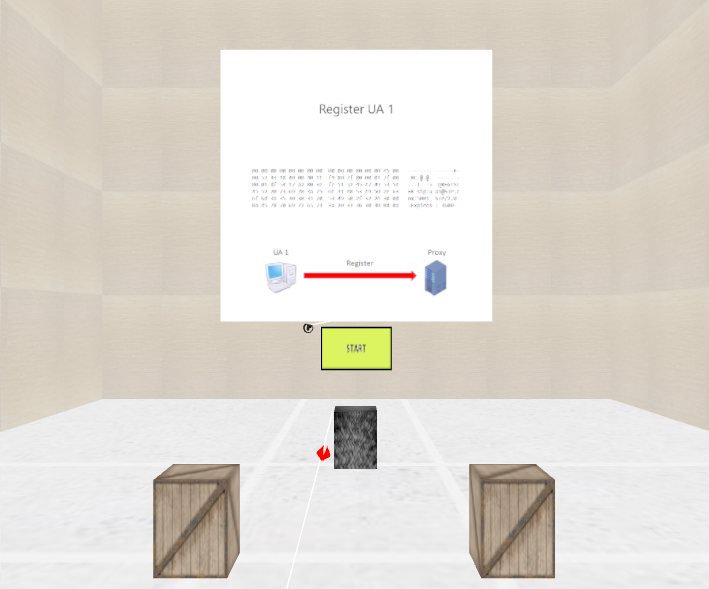
\includegraphics[width=12cm, keepaspectratio]{img/resultados/01-Register_UA1.PNG}
  \caption{Mensaje de registro inicial de UA1}
  \label{fig:01-Register_UA1}
\end{figure}
\clearpage

Si el usuario no está autorizado, recibe un mensaje 401 UNAUTHORIZED, mostrado en la figura~\ref{fig:02-Unauthorized}. 

El mensaje 401 UNAUTHORIZED es una respuesta del servidor que indica que el intento de registro ha fallado debido a la falta de 
credenciales adecuadas. Como resultado, el usuario (UA1) debe realizar otro intento de REGISTER con la información de autenticación 
adecuada, como un nombre de usuario y una contraseña válidos.

\bigskip

\begin{figure}[H]
  \centering
  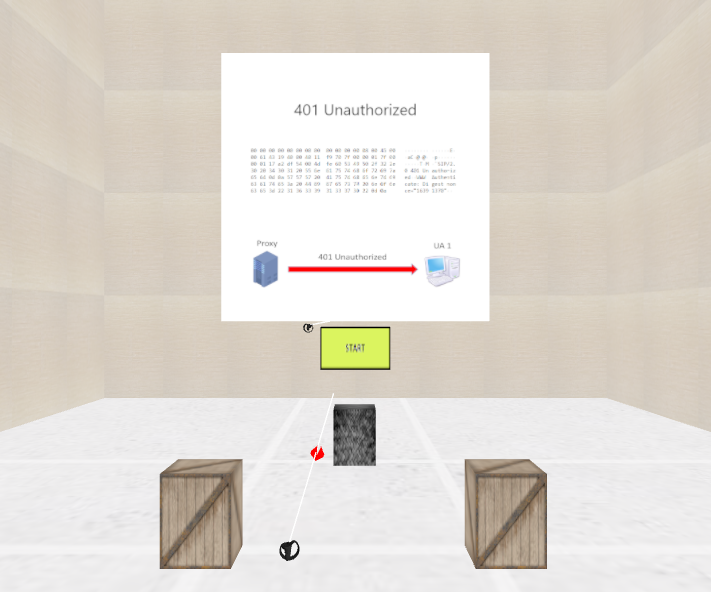
\includegraphics[width=12cm, keepaspectratio]{img/resultados/02-Unautorized.PNG}
  \caption{Respuesta 401 UNAUTHORIZED a UA1}
  \label{fig:02-Unauthorized}
\end{figure}
\clearpage

El segundo intento de REGISTER es aceptado y confirmado con una respuesta 200 OK, ilustrado en la figura~\ref{fig:03-200OK}. 

El mensaje 200 OK indica que el servidor ha aceptado el registro del usuario y que el usuario está ahora autenticado y registrado en el sistema. 
Este mensaje puede incluir información adicional de los parámetros de configuración de la sesión.

\bigskip

\begin{figure}[H]
  \centering
  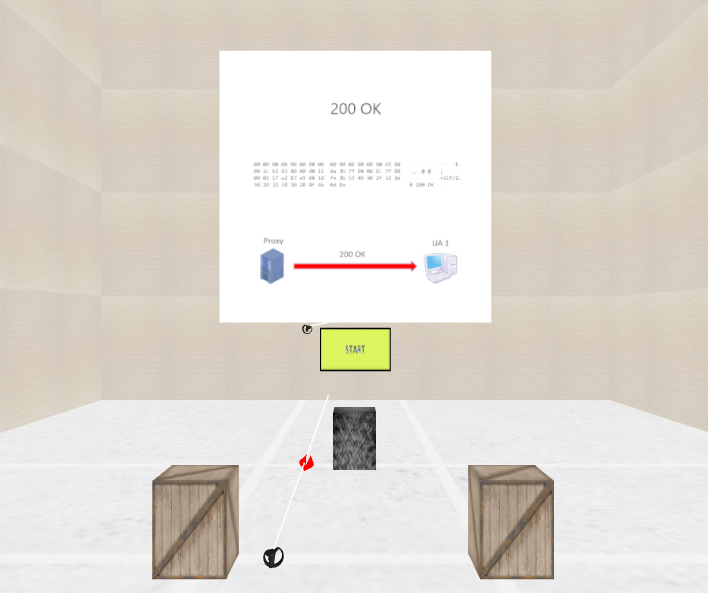
\includegraphics[width=12cm, keepaspectratio]{img/resultados/02-200OK.PNG}
  \caption{Registro de UA1 exitoso con 200 OK}
  \label{fig:03-200OK}
\end{figure}
\clearpage

A continuación, el usuario B (UA2) se registra enviando un mensaje REGISTER al servidor,
representado en la figura~\ref{fig:04-Register_UA2}. Este mensaje sigue el mismo proceso de autenticación y registro. 

La figura muestra cómo UA2 inicia el proceso de registro proporcionando su información de autenticación al servidor.

\bigskip

\begin{figure}[H]
  \centering
  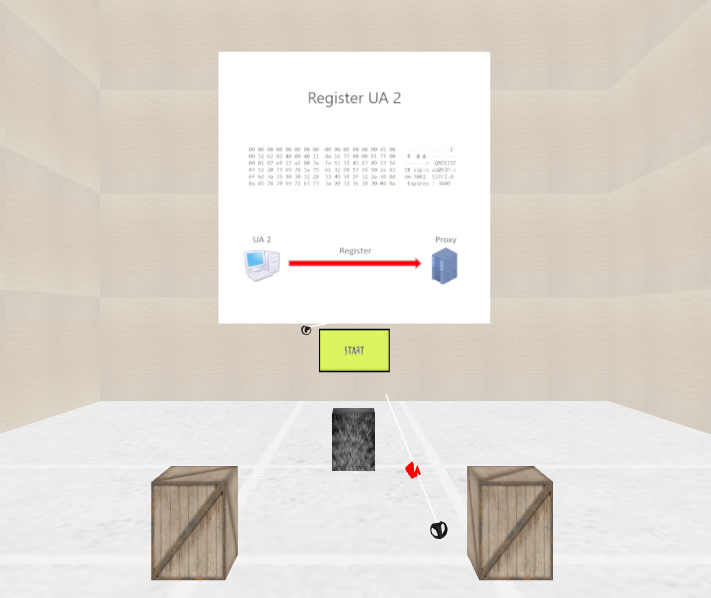
\includegraphics[width=12cm, keepaspectratio]{img/resultados/03-Register_UA2.PNG}
  \caption{Mensaje de registro inicial de UA2}
  \label{fig:04-Register_UA2}
\end{figure}
\clearpage

El registro de UA2 es aceptado y confirmado con una respuesta 200 OK, ilustrado en la figura~\ref{fig:05-200OK_UA2}. 

De igual forma que en registro de UA1, el mensaje 200 OK confirma que UA2 ha sido autenticado y registrado exitosamente en el sistema.

\bigskip

\begin{figure}[H]
  \centering
  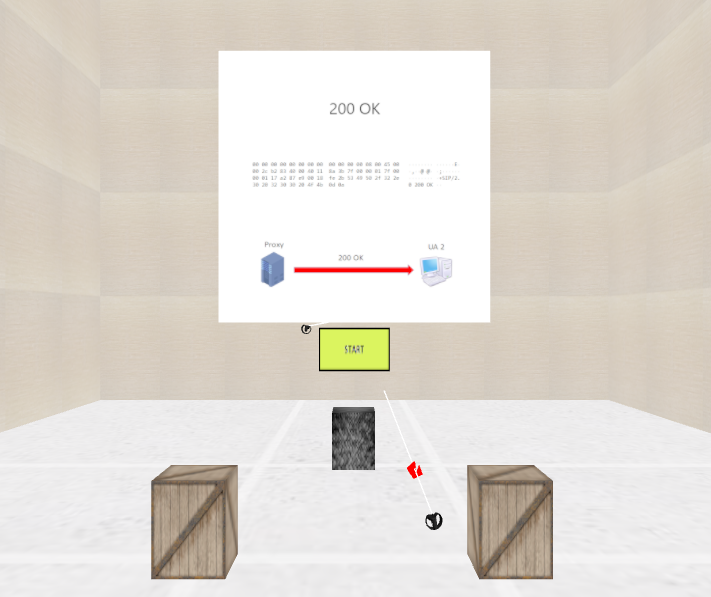
\includegraphics[width=12cm, keepaspectratio]{img/resultados/04-200OK.PNG}
  \caption{Registro de UA2 exitoso con 200 OK}
  \label{fig:05-200OK_UA2}
\end{figure}
\clearpage

Ahora que ambos usuarios están registrados en el servidor proxy, la fase de llamada comienza con un mensaje INVITE acompañado de 
una descripción de la sesión (SDP), escenificado en la figura~\ref{fig:06-Invite}. 

El mensaje INVITE es enviado por UA1 a UA2 a través del servidor y contiene detalles sobre la sesión propuesta, 
incluyendo los parámetros de conexión.

\bigskip

\begin{figure}[H]
  \centering
  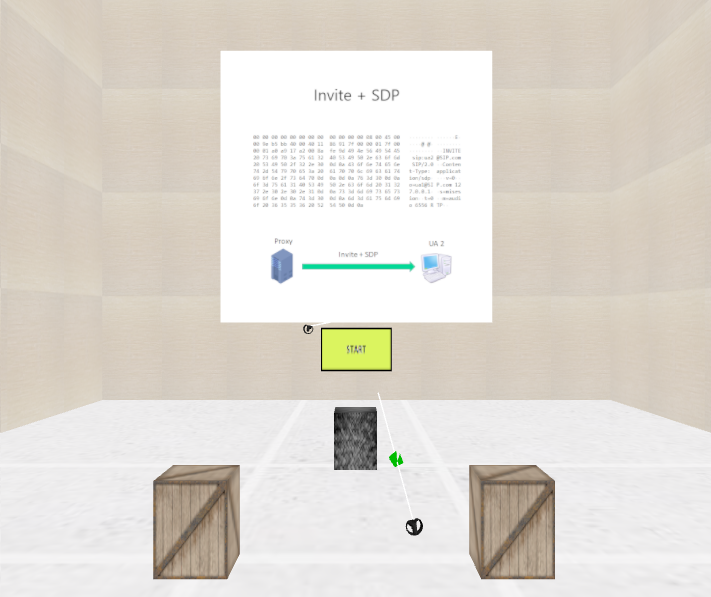
\includegraphics[width=12cm, keepaspectratio]{img/resultados/06-Invite.PNG}
  \caption{Inicio de llamada con el mensaje INVITE de UA1}
  \label{fig:06-Invite}
\end{figure}
\clearpage

Este mensaje es respondido con un 100 TRYING, evidenciado en la figura~\ref{fig:07-Trying}. 
El mensaje 100 TRYING indica que el servidor ha recibido el mensaje INVITE y está intentando localizar al usuario de destino (UA2).

Posteriormente, el servidor envía un 180 RINGING, ilustrado en la figura~\ref{fig:08-Ringing}, 
que indica que la llamada está siendo procesada y que el otro usuario está siendo alertado de la llamada entrante.

\begin{figure}[H]
  \centering
  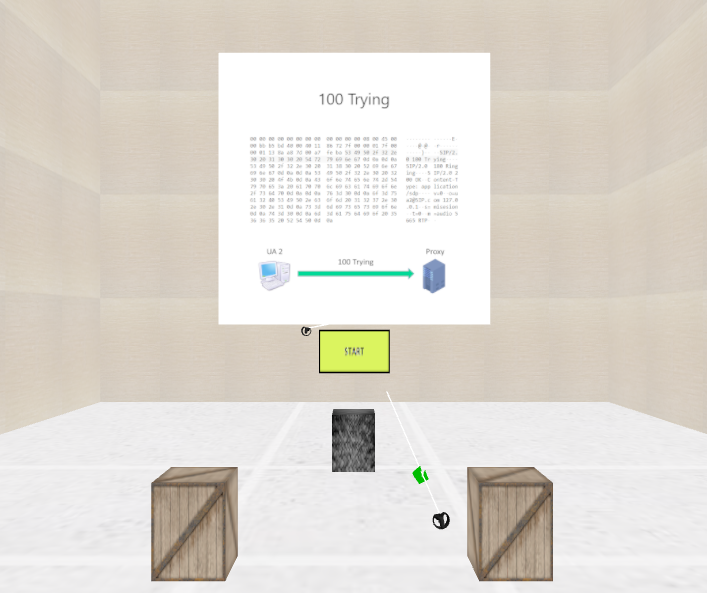
\includegraphics[width=9cm, keepaspectratio]{img/resultados/07-Trying.PNG}
  \caption{Respuesta TRYING de UA2 indicando procesamiento}
  \label{fig:07-Trying}
\end{figure}

\begin{figure}[H]
  \centering
  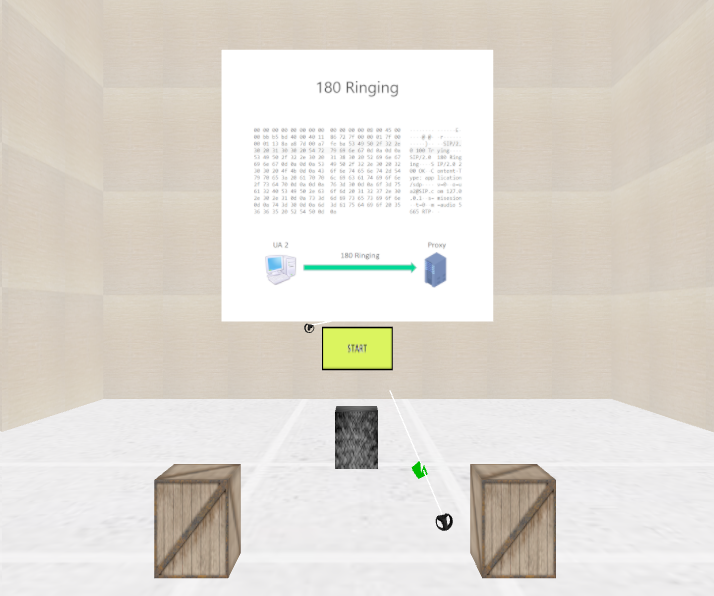
\includegraphics[width=9cm, keepaspectratio]{img/resultados/08-Ringing.PNG}
  \caption{Alerta de llamada con el mensaje RINGING de UA2}
  \label{fig:08-Ringing}
\end{figure}
\clearpage

Cuando el usuario B (UA2) acepta la llamada, envía una respuesta 200 OK + SDP, representado en la figura~\ref{fig:09-200OKSDP}. 

Este mensaje contiene la confirmación de que UA2 está listo para establecer la sesión de comunicación y proporciona los detalles 
necesarios para la transmisión.

\bigskip

\begin{figure}[H]
  \centering
  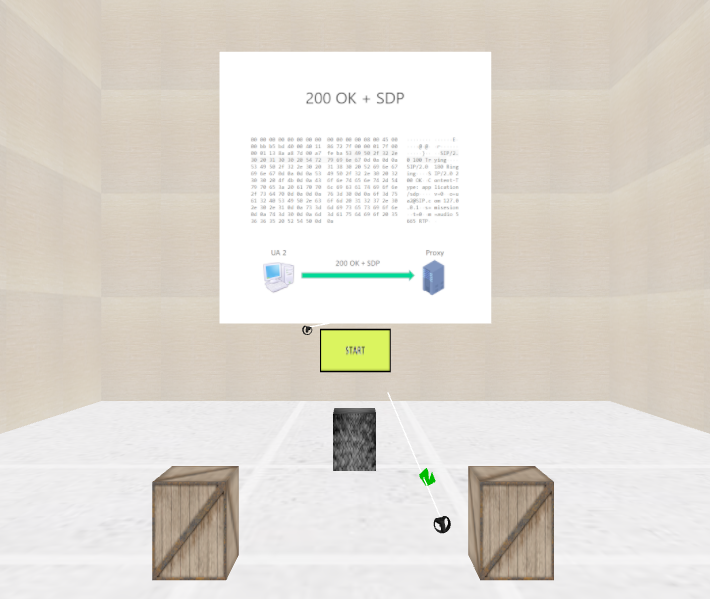
\includegraphics[width=12cm, keepaspectratio]{img/resultados/09-200OKSDP.PNG}
  \caption{Confirmación de llamada con 200 OK + SDP de UA2}
  \label{fig:09-200OKSDP}
\end{figure}
\clearpage

El usuario A (UA1) confirma recibir esta información con un ACK, mostrado en la figura~\ref{fig:10-ACK}. 

El mensaje ACK es una confirmación final que completa el establecimiento de la llamada y permite el inicio de la transmisión.

\bigskip

\begin{figure}[H]
  \centering
  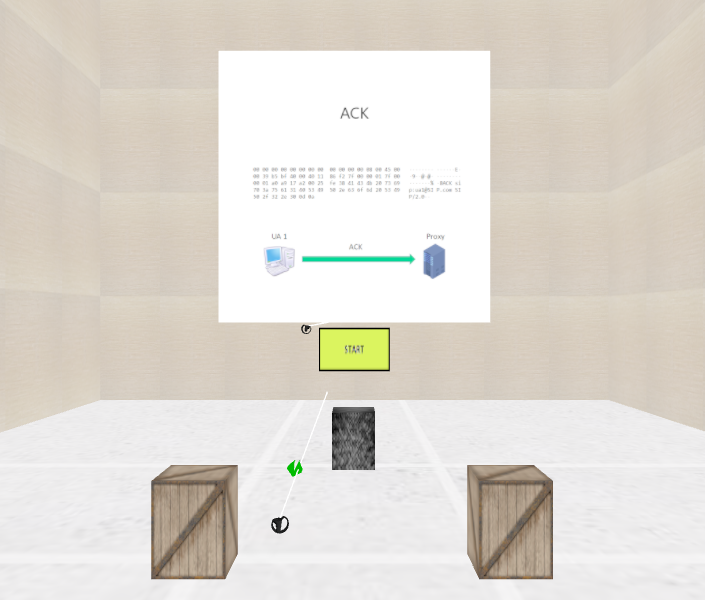
\includegraphics[width=12cm, keepaspectratio]{img/resultados/13-ACK.PNG}
  \caption{Reconocimiento ACK de UA1 completando el establecimiento de la llamada}
  \label{fig:10-ACK}
\end{figure}
\clearpage

Una vez establecida la llamada, los datos multimedia se transmiten a través de 
paquetes RTP (Protocolo de Transporte en Tiempo Real), escenificado en la figura~\ref{fig:11-RTP}. 

Los paquetes RTP transportan la información de audio entre UA1 y UA2, permitiendo la comunicación en tiempo real.

\bigskip

\begin{figure}[H]
  \centering
  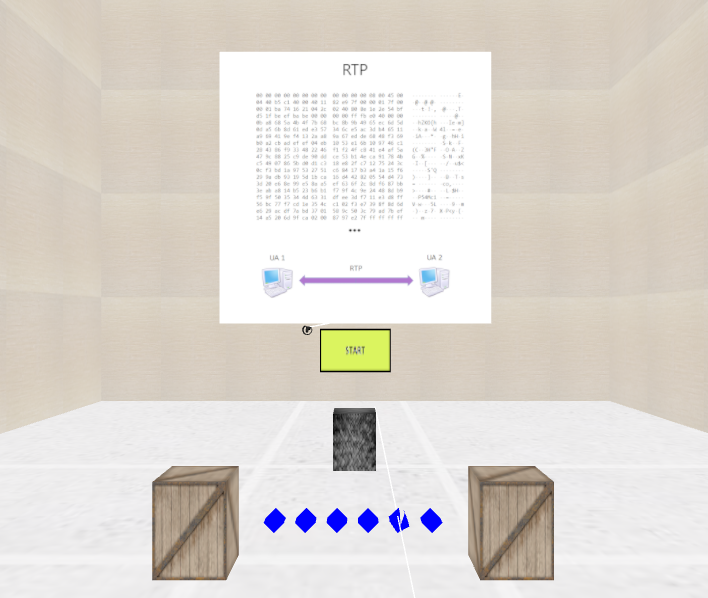
\includegraphics[width=12cm, keepaspectratio]{img/resultados/15-RTP.PNG}
  \caption{Transmisión de datos multimedia a través de paquetes RTP}
  \label{fig:11-RTP}
\end{figure}
\clearpage

Este intercambio continúa hasta que uno de los usuarios decide terminar la llamada, 
enviando un mensaje BYE, ilustrado en la figura~\ref{fig:12-BYE}. 

El mensaje BYE indica la intención de finalizar la llamada y cerrar la sesión de comunicación.

\bigskip

\begin{figure}[H]
  \centering
  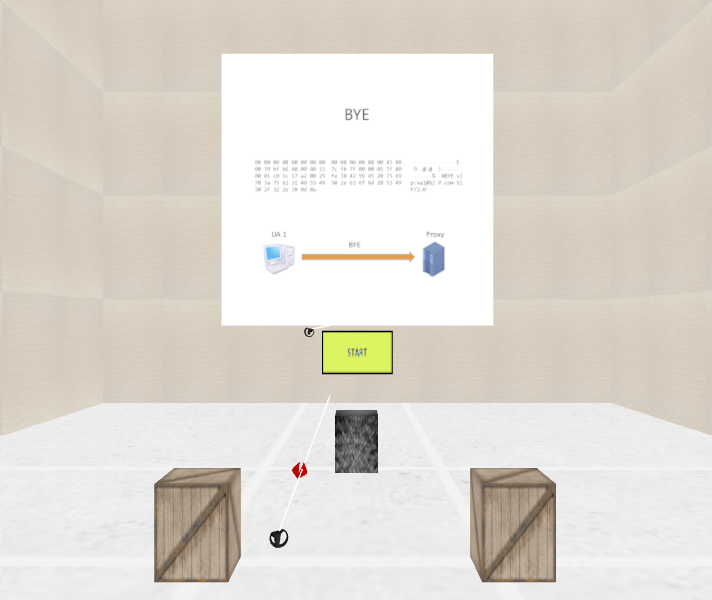
\includegraphics[width=12cm, keepaspectratio]{img/resultados/16-BYE.PNG}
  \caption{Mensaje BYE enviado para terminar la llamada}
  \label{fig:12-BYE}
\end{figure}
\clearpage

El fin de la llamada es confirmado por el otro usuario con un 200 OK, representado en la figura~\ref{fig:13-200OK_BYE}, 
cerrando así la sesión de comunicación. 

Este mensaje final confirma que ambos usuarios han terminado la sesión de manera ordenada.

\bigskip

\begin{figure}[H]
  \centering
  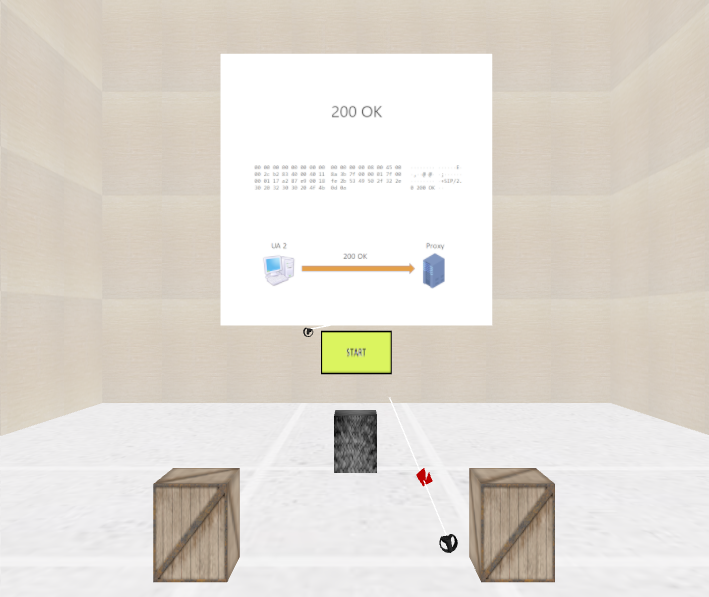
\includegraphics[width=12cm, keepaspectratio]{img/resultados/18-200OK.PNG}
  \caption{Confirmación del fin de la llamada con un 200 OK}
  \label{fig:13-200OK_BYE}
\end{figure}


%%%%%%%%%%%%%%%%%%%%%%%%%%%%%%%%%%%%%%%%%%%%%%%%%%%%%%%%%%%%%%%%%%%%%%%%%%%%%%%%
%%%%%%%%%%%%%%%%%%%%%%%%%%%%%%%%%%%%%%%%%%%%%%%%%%%%%%%%%%%%%%%%%%%%%%%%%%%%%%%%
% CONCLUSIONES %
%%%%%%%%%%%%%%%%%%%%%%%%%%%%%%%%%%%%%%%%%%%%%%%%%%%%%%%%%%%%%%%%%%%%%%%%%%%%%%%%

\cleardoublepage
\chapter{Conclusiones}
\label{chap:conclusiones}


\section{Consecución de objetivos}
\label{sec:consecucion-objetivos}

\subsection{Objetivo general}
El objetivo general del proyecto era construir una representación visual y funcional de los flujos de señalización y 
datos en un entorno de realidad virtual, utilizando tecnologías avanzadas como Three.js y módulos adicionales para facilitar 
la interacción en entornos VR. Este objetivo se ha cumplido satisfactoriamente, como se demostró en los resultados de funcionamiento 
del sistema, donde los usuarios pueden interactuar con la simulación de comunicaciones y experimentar de forma inmersiva el manejo de 
las comunicaciones en tiempo real.


\section{Aplicación de lo aprendido}
\label{sec:aplicacion}

A lo largo de mi formación en el grado de Ingeniería en Sistemas Audiovisuales y Multimedia, adquirí una serie de conocimientos y 
habilidades que han sido fundamentales para el desarrollo de mi proyecto de fin de grado. A continuación, detallo cómo se aplicaron 
específicamente algunas de las asignaturas más relevantes:

\begin{enumerate}
  \item \textbf{Informática I e Informática II:} Estas fueron las primeras asignaturas relacionadas con la programación, 
  las cuales sentaron las bases y aportaron los primeros pasos para desarrollar habilidades en el área de las telecomunicaciones.
  \item \textbf{Protocolos para la Transmisión de Audio y Vídeo por Internet:} Esta asignatura profundizó en la programación de manera 
  más específica, realizando prácticas que combinaban conocimientos técnicos con la utilización de protocolos de comunicación.
  \item \textbf{Construcción de Servicios y Aplicaciones Audiovisuales en Internet:} En esta asignatura se asentaron las bases del desarrollo 
  web utilizando lenguajes como JavaScript, HTML5 y CSS, elementos cruciales para la interfaz de usuario de mi proyecto.
  \item \textbf{Gráficos y Visualización en 3D:} Aprendí a desarrollar una parte significativa de mi proyecto, adquiriendo conocimientos en 
  gráficos 3D, conceptos básicos de WebGL y la creación de gráficos utilizando Three.js.
\end{enumerate}

En general, todas las asignaturas del grado han aportado valiosos conocimientos y fomentado el desarrollo del pensamiento crítico y la resolución de problemas, habilidades que he aplicado tanto en el TFG como en el entorno laboral.

\section{Lecciones aprendidas}
\label{sec:lecciones_aprendidas}

Durante el desarrollo de este proyecto, he adquirido una serie de conocimientos tanto técnicos como personales que han enriquecido 
mi experiencia y han contribuido a mi desarrollo profesional.

\begin{enumerate}
\item \textbf{Importancia de la planificación detallada:} Una de las lecciones más valiosas ha sido comprender la importancia de una planificación 
y organización en proyectos de desarrollo tecnológico.

\item \textbf{Profundización en tecnologías de realidad virtual:} El proyecto me permitió profundizar en el uso de tecnologías de realidad virtual, 
especialmente en la programación con JavaScript y el uso de bibliotecas como Three.js. Aprendí no solo a implementar estas tecnologías sino también 
a resolver problemas específicos relacionados con la renderización de gráficos 3D y la interactividad en entornos virtuales~\cite{Ejemplos_Three.js}.

\item \textbf{Capacidad de adaptación y solución de problemas:} Desarrollo de la capacidad de buscar soluciones alternativas y adaptar el enfoque del proyecto según las 
circunstancias fue importante para el éxito del proyecto.

\item \textbf{Comprensión de los protocolos de comunicación:} El proyecto profundizó mi comprensión de los protocolos de comunicación como SIP y RTP. 
A través de la implementación práctica, pude ver cómo la teoría se aplica en situaciones reales.
\end{enumerate}


\section{Trabajos futuros}
\label{sec:trabajos_futuros}

Los resultados obtenidos implican que la aplicación de realidad virtual en el campo de las telecomunicaciones puede mejorar 
significativamente la comprensión de sistemas complejos de comunicación. Se recomienda que investigaciones futuras exploren 
ampliar la funcionalidad del sistema para incluir más escenarios de comunicación y evaluar su 
aplicabilidad en entornos educativos y profesionales.


%%%%%%%%%%%%%%%%%%%%%%%%%%%%%%%%%%%%%%%%%%%%%%%%%%%%%%%%%%%%%%%%%%%%%%%%%%%%%%%%
%%%%%%%%%%%%%%%%%%%%%%%%%%%%%%%%%%%%%%%%%%%%%%%%%%%%%%%%%%%%%%%%%%%%%%%%%%%%%%%%
% APÉNDICE(S) %
%%%%%%%%%%%%%%%%%%%%%%%%%%%%%%%%%%%%%%%%%%%%%%%%%%%%%%%%%%%%%%%%%%%%%%%%%%%%%%%%

\cleardoublepage
\appendix
\chapter{Manual de usuario}
\label{app:manual}

Este apéndice proporciona un manual de usuario para la aplicación desarrollada en este proyecto. 
Aquí se explican los pasos para instalar, configurar y utilizar la aplicación.

\section{Requisitos del sistema}
Para utilizar esta aplicación, asegúrate de que tu sistema cumple con los siguientes requisitos:
\begin{itemize}
    \item Sistema operativo: Windows.
    \item Navegador web compatible: Google Chrome.
    \item Hardware: Gafas de realidad virtual (por ejemplo, Oculus Quest 2) o en su defecto, descargarse la extensión Web XR API Emulator.
    \item Conexión a Internet.
\end{itemize}

\section{Uso de la aplicación}
\subsection{Instalación de la extensión WebXR API Emulator}
Lo primero que debemos hacer es descargarnos e instalar la extensión 
Web XR API Emulator.

Una vez realizado este paso, accedemos a la URL donde se encuentra 
desplegada la aplicación. La URL es la siguiente:

\url{https://jorgegragon.github.io/TFGJorge/VRM/index.html}


\subsection{Activación de la realidad virtual}
A continuación pulsamos F12 para abrir la herramienta de desarrollador, 
donde seleccionaremos en la parte superior de esta ventana, la opción de WebXR.

Una vez realizado este paso, en la parte inferior de la escena, tenemos 
un botón que pone Enter VR. Lo pulsamos para activar la realidad virtual.

\subsection{Interacción en la aplicación}
Ya tenemos la aplicación funcionando, podremos movernos por la escena, 
accionar botones y obtener información acerca de los usuarios y del proxy.

Tenemos dos controles, que producen interacción con la aplicación:
\begin{itemize}
  \item \textbf{Select Button del controlador izquierdo:} Con este botón nos movemos por la escena en la dirección frontal hacia donde están mirando las gafas virtuales.
  \item \textbf{Select Button del controlador derecho:} Con este botón interactuamos con los objetos de la escena. Apuntamos 
  hacia el objeto y pulsamos el botón. Esto hará que, dependiendo del 
  objeto seleccionado, se produzca o no un cambio en la escena.
\end{itemize}

\subsection{Activación de la secuencia de intercambio de paquetes}
Para activar la secuencia del intercambio de paquetes, con el controlador derecho, 
apuntar hacia el botón de START y pulsamos el Select Button.

De esta forma, veremos cómo se ejecuta el intercambio, pudiendo pararlo en todo 
momento para obtener información de los paquetes, usuarios o proxy, de la misma 
forma que hemos
hecho anteriormente, ya que el botón en la escena que indicaba START ahora 
indicará STOP.

\section{Modo sin realidad virtual}
Si no se desea ejecutar la aplicación en realidad virtual, no se quiere descargar la extensión, o no se poseen gafas VR, se puede visualizar la escena y 
el intercambio de paquetes en 2D utilizando los controles del teclado en la siguiente URL:

\url{https://jorgegragon.github.io/TFGJorge/Original/AreaEstado.html}

Donde los controles serán:

\begin{itemize}
  \item \textbf{Movimiento:} W, A, S, D, Q y E
  \item \textbf{Iniciar secuencia:} Usar la barra espaciadora para comenzar el intercambio.
  \item \textbf{Parar secuencia:} Clicar en los usuarios, proxy o paquete.
  \item \textbf{Reanudar secuencia:} Usar la barra espaciadora para reanudar.
\end{itemize}

\cleardoublepage

\bibliographystyle{abbrv}
\bibliography{memoria_JorgeGrande}

\end{document}
